% Options for packages loaded elsewhere
% Options for packages loaded elsewhere
\PassOptionsToPackage{unicode}{hyperref}
\PassOptionsToPackage{hyphens}{url}
\PassOptionsToPackage{dvipsnames,svgnames,x11names}{xcolor}
%
\documentclass[
  authoryear,
  doubleblind,
  3p]{elsarticle}
\usepackage{xcolor}
\usepackage{amsmath,amssymb}
\setcounter{secnumdepth}{-\maxdimen} % remove section numbering
\usepackage{iftex}
\ifPDFTeX
  \usepackage[T1]{fontenc}
  \usepackage[utf8]{inputenc}
  \usepackage{textcomp} % provide euro and other symbols
\else % if luatex or xetex
  \usepackage{unicode-math} % this also loads fontspec
  \defaultfontfeatures{Scale=MatchLowercase}
  \defaultfontfeatures[\rmfamily]{Ligatures=TeX,Scale=1}
\fi
\usepackage{lmodern}
\ifPDFTeX\else
  % xetex/luatex font selection
\fi
% Use upquote if available, for straight quotes in verbatim environments
\IfFileExists{upquote.sty}{\usepackage{upquote}}{}
\IfFileExists{microtype.sty}{% use microtype if available
  \usepackage[]{microtype}
  \UseMicrotypeSet[protrusion]{basicmath} % disable protrusion for tt fonts
}{}
\makeatletter
\@ifundefined{KOMAClassName}{% if non-KOMA class
  \IfFileExists{parskip.sty}{%
    \usepackage{parskip}
  }{% else
    \setlength{\parindent}{0pt}
    \setlength{\parskip}{6pt plus 2pt minus 1pt}}
}{% if KOMA class
  \KOMAoptions{parskip=half}}
\makeatother
% Make \paragraph and \subparagraph free-standing
\makeatletter
\ifx\paragraph\undefined\else
  \let\oldparagraph\paragraph
  \renewcommand{\paragraph}{
    \@ifstar
      \xxxParagraphStar
      \xxxParagraphNoStar
  }
  \newcommand{\xxxParagraphStar}[1]{\oldparagraph*{#1}\mbox{}}
  \newcommand{\xxxParagraphNoStar}[1]{\oldparagraph{#1}\mbox{}}
\fi
\ifx\subparagraph\undefined\else
  \let\oldsubparagraph\subparagraph
  \renewcommand{\subparagraph}{
    \@ifstar
      \xxxSubParagraphStar
      \xxxSubParagraphNoStar
  }
  \newcommand{\xxxSubParagraphStar}[1]{\oldsubparagraph*{#1}\mbox{}}
  \newcommand{\xxxSubParagraphNoStar}[1]{\oldsubparagraph{#1}\mbox{}}
\fi
\makeatother


\usepackage{longtable,booktabs,array}
\usepackage{calc} % for calculating minipage widths
% Correct order of tables after \paragraph or \subparagraph
\usepackage{etoolbox}
\makeatletter
\patchcmd\longtable{\par}{\if@noskipsec\mbox{}\fi\par}{}{}
\makeatother
% Allow footnotes in longtable head/foot
\IfFileExists{footnotehyper.sty}{\usepackage{footnotehyper}}{\usepackage{footnote}}
\makesavenoteenv{longtable}
\usepackage{graphicx}
\makeatletter
\newsavebox\pandoc@box
\newcommand*\pandocbounded[1]{% scales image to fit in text height/width
  \sbox\pandoc@box{#1}%
  \Gscale@div\@tempa{\textheight}{\dimexpr\ht\pandoc@box+\dp\pandoc@box\relax}%
  \Gscale@div\@tempb{\linewidth}{\wd\pandoc@box}%
  \ifdim\@tempb\p@<\@tempa\p@\let\@tempa\@tempb\fi% select the smaller of both
  \ifdim\@tempa\p@<\p@\scalebox{\@tempa}{\usebox\pandoc@box}%
  \else\usebox{\pandoc@box}%
  \fi%
}
% Set default figure placement to htbp
\def\fps@figure{htbp}
\makeatother





\setlength{\emergencystretch}{3em} % prevent overfull lines

\providecommand{\tightlist}{%
  \setlength{\itemsep}{0pt}\setlength{\parskip}{0pt}}



 
\usepackage[]{natbib}
\bibliographystyle{elsarticle-harv}


\usepackage{xcolor}
\definecolor{revgreen}{HTML}{228B22}

% Block version (paragraphs)
\newenvironment{revision}{\color{revgreen}}{}

% Inline version (phrases/sentences, safe with citations)
\DeclareRobustCommand{\rev}[1]{{\color{revgreen}#1}}
\usepackage{booktabs}
\usepackage{longtable}
\usepackage{array}
\usepackage{multirow}
\usepackage{wrapfig}
\usepackage{float}
\usepackage{colortbl}
\usepackage{pdflscape}
\usepackage{tabu}
\usepackage{threeparttable}
\usepackage{threeparttablex}
\usepackage[normalem]{ulem}
\usepackage{makecell}
\usepackage{xcolor}
\usepackage{setspace}
\onehalfspacing
\geometry{margin=1in}
\usepackage{todonotes,mathtools,bm,amsmath,mathpazo}
\usepackage[linesnumbered,ruled,vlined]{algorithm2e}
\setlength{\parindent}{0cm}
\usepackage{tikz}
\usetikzlibrary{
    arrows.meta,
    positioning,
    fit,
    calc,
    shapes.misc,
    shapes.multipart
  }
\makeatletter
\@ifpackageloaded{caption}{}{\usepackage{caption}}
\AtBeginDocument{%
\ifdefined\contentsname
  \renewcommand*\contentsname{Table of contents}
\else
  \newcommand\contentsname{Table of contents}
\fi
\ifdefined\listfigurename
  \renewcommand*\listfigurename{List of Figures}
\else
  \newcommand\listfigurename{List of Figures}
\fi
\ifdefined\listtablename
  \renewcommand*\listtablename{List of Tables}
\else
  \newcommand\listtablename{List of Tables}
\fi
\ifdefined\figurename
  \renewcommand*\figurename{Figure}
\else
  \newcommand\figurename{Figure}
\fi
\ifdefined\tablename
  \renewcommand*\tablename{Table}
\else
  \newcommand\tablename{Table}
\fi
}
\@ifpackageloaded{float}{}{\usepackage{float}}
\floatstyle{ruled}
\@ifundefined{c@chapter}{\newfloat{codelisting}{h}{lop}}{\newfloat{codelisting}{h}{lop}[chapter]}
\floatname{codelisting}{Listing}
\newcommand*\listoflistings{\listof{codelisting}{List of Listings}}
\makeatother
\makeatletter
\makeatother
\makeatletter
\@ifpackageloaded{caption}{}{\usepackage{caption}}
\@ifpackageloaded{subcaption}{}{\usepackage{subcaption}}
\makeatother
\journal{Production and Operations Management}
\usepackage{bookmark}
\IfFileExists{xurl.sty}{\usepackage{xurl}}{} % add URL line breaks if available
\urlstyle{same}
\hypersetup{
  pdftitle={E-companion to Estimating censored demand in family planning supply chains: forecast accuracy, inventory implications, and public health outcomes},
  colorlinks=true,
  linkcolor={blue},
  filecolor={Maroon},
  citecolor={Blue},
  urlcolor={Blue},
  pdfcreator={LaTeX via pandoc}}


\setlength{\parindent}{6pt}
\begin{document}
% Typeset the E-companion title without the Elsevier front matter.
\begingroup
\centering
\singlespacing
\Large\bfseries
E-companion to Estimating censored demand in family planning supply
chains: forecast accuracy, inventory implications, and public health
outcomes\par
\endgroup
\vspace{0.8em}

\subsection{Section 1: Truncated log-likelihood and parameter
initialisation}\label{sec-appendix_wp2_1}

The derivation of the likelihood function begins by noting that, prior
to censoring, the one-step-ahead forecast error for each observation
follows a normal distribution:

\begin{equation}\phantomsection\label{eq-wp2_a1}{
y_t \mid \mathcal{F}_{t-1} \sim \mathcal{N}(\mu_t, \sigma_t^2)
}\end{equation}

where \(\mu_t = H \hat{X}_{t|t-1}\) and
\(\sigma_t^2 = H P_{t|t-1} H^\top + R\) are the predicted mean and
variance at time \(t\), conditional on prior information
\(\mathcal{F}_{t-1}\).

However, due to stock constraints, the observed values may be censored.
Accordingly, we distinguish three regimes:

\begin{itemize}
\item
  \textbf{Uncensored}: The full observation \(y_t\) is available. The
  likelihood is the usual Gaussian density:

  \begin{equation}\phantomsection\label{eq-wp2_a2}{
  p(y_t \mid \mu_t, \sigma_t^2) = \frac{1}{\sqrt{2\pi \sigma_t^2}} \exp\left( -\frac{(y_t - \mu_t)^2}{2\sigma_t^2} \right)
  }\end{equation}
\item
  \textbf{Partially censored}: We observe \(y_t = \min(D_t, s_t)\), and
  know that true demand exceeds the observed value. This is equivalent
  to right-censoring from below at \(y_t\), and the likelihood becomes
  the survival function:

  \begin{equation}\phantomsection\label{eq-wp2_a3}{
  P(Y_t > y_t) = 1 - \Phi\left( \frac{y_t - \mu_t}{\sigma_t} \right)
  }\end{equation}
\item
  \textbf{Fully censored}: For \(y_t = 0\), the only information
  available is that demand is positive but completely unobserved due to
  stockouts or interruptions. The likelihood in this case becomes:

  \[
  P(Y_t > 0) = 1 - \Phi\left( -\frac{\mu_t}{\sigma_t} \right)
  \]
\end{itemize}

Taking logs and summing over time leads to the total log-likelihood:

\begin{equation}\phantomsection\label{eq-wp2_a4}{
\log L(\theta) = \sum_t \log p(y_t \mid \mu_t, \sigma_t^2)
}\end{equation}

which, depending on the censoring status of each observation, expands
to:

\begin{equation}\phantomsection\label{eq-wp2_a5}{
\log L(\theta) = \sum_t
\begin{cases}
-\frac{1}{2} \left[ \log(2\pi \sigma_t^2) + \frac{(y_t - \mu_t)^2}{\sigma_t^2} \right], & \text{if } y_t \text{ is uncensored} \\
\log\left(1 - \Phi\left(\frac{y_t - \mu_t}{\sigma_t}\right)\right), & \text{if } y_t \text{ is partially censored} \\
\log\left(1 - \Phi\left(-\frac{\mu_t}{\sigma_t}\right)\right), & \text{if } y_t = 0 \text{ (fully censored)}
\end{cases}
}\end{equation}

Each term in this expression corresponds to the conditional probability
of observing \(y_t\) given the predicted distribution under the Kalman
framework. For uncensored observations, the log-likelihood follows the
Gaussian log-density, directly comparing the observed and predicted
values. In the partially censored case, the observation is known only to
lie above the censored threshold; thus, its likelihood is the log of the
survival function of the normal distribution. For fully censored points,
where \(y_t = 0\), we only know that the true demand exceeded zero. This
results in a likelihood based solely on the left tail of the predicted
Gaussian distribution.

\subsubsection{Initialization and parameter
estimation}\label{initialization-and-parameter-estimation}

\subsubsection{Initializing state
vector}\label{initializing-state-vector}

The latent state vector \(X_0 = (\ell_0, \tau_0, \gamma_0)^T\) includes
the level, trend, and seasonal components. To initialize \(X_0\), we
rely on a training subset of the data containing uncensored
observations. This subset is first decomposed using STL (Seasonal-Trend
decomposition via Loess) \citep{cleveland1990}, from which the initial
values are extracted:

\begin{itemize}
\tightlist
\item
  \(\ell_0\): set to the most recent value of the STL trend component
\item
  \(\tau_0\): estimated as the average slope over a small rolling window
  in the trend component
\item
  \(\gamma_0\): set to the final value of the seasonal component from
  STL or the mean of a complete seasonal cycle if available
\end{itemize}

In cases where no seasonal pattern is reliable at initialization,
\(\gamma_0\) is set to zero and learned adaptively.

These initializations follow standard practices in state-space modeling
\citep{durbin2012, harvey1990}, where the latent level and trend are
derived from available smoothed signals to provide a statistically
grounded prior. Phase alignment in the seasonal component initialization
ensures consistency with the observed seasonal structure when available
\citep{harvey1990}.

\subsubsection{Initializing covariance
matrix}\label{initializing-covariance-matrix}

In line with recommendations for initializing latent state uncertainty
under partial observability \citep{west1997}, the initial state
covariance matrix \(P_{0|0}\) is defined as a diagonal matrix with
variances estimated from the empirical variance of each corresponding
STL component:

\begin{equation}\phantomsection\label{eq-eleven}{
P_{0|0} = \text{diag}(\sigma^2_{\ell},\ \sigma^2_{\tau},\ \sigma^2_{\gamma})
}\end{equation}

This specification captures component-specific volatility while assuming
independence between state dimensions at initialization. If no reliable
estimation is available, we specify a high-variance diffuse prior (e.g.,
variance of 100) to allow sufficient flexibility in early state
adaptation.

\subsubsection{Initializing parameters}\label{initializing-parameters}

The parameters \(Q_0, R, \phi\) and \(\lambda\) are initialized as
follows:

\begin{itemize}
\tightlist
\item
  \(Q_0 = \text{diag}(0.1, 0.1, 0.1)\): assumes gradual independent
  evolution across components \citep{harvey1990}
\item
  \(R\): initialized based on the variance of residuals obtained from
  STL decomposition \citep{durbin2012}
\item
  \(\phi\): set to 0.9 to allow persistence in seasonal patterns
  \citep{west1997}
\item
  \(\lambda\): initialized to 0.5 to model moderate inflation of
  uncertainty during censoring, aligned with the dynamic variance
  inflation strategies discussed in \citet{trapero2024}
\end{itemize}

These initial values are subsequently refined through maximizing the
truncated log-likelihood:

\begin{equation}\phantomsection\label{eq-twelve}{
\log \mathcal{L}(\theta) = \sum_t \begin{cases}
  -\frac{1}{2} \left[ \log(\sigma_t^2) + \frac{(y_t - \mu_t)^2}{\sigma_t^2} \right] & \text{if uncensored} \\
  \log \left(1 - \Phi\left(\frac{y_t - \mu_t}{\sigma_t}\right)\right) & \text{if partially censored} \\
  \log \left(1 - \Phi\left(\frac{-\mu_t}{\sigma_t} \right)\right), & \text{if fully censored (i.e., } y_t = 0\text{)}
\end{cases}
}\end{equation}

\pagebreak

\pagebreak

\subsection{Section 2: Forecasting methods}\label{sec-appendix_wp2_2}

\subsubsection{Naive}\label{naive}

This method is a simple forecasting approach that uses the last observed
demand as the forecast for future periods. It's often used as a basic
benchmark in time series forecasting to compare how well more complex
methods perform \citep{kolassa2023}. The Naive forecast for \(h\) steps
ahead is calculated as the most recent actual observation \(y_t\):

\begin{equation}\phantomsection\label{eq-naive_wp2}{
\hat{y}_{t+h|t} = y_t
}\end{equation}

We used the NAIVE() function from the \emph{fable} package in R to
implement this method \citep{fable2022}.

\subsubsection{Mean}\label{mean}

In the Mean method, forecasts are generated by taking the average of
historical data over a fixed window \citep{hyndman2021forecasting}. So,
the Mean forecast for \(h\) steps ahead using \(k\) periods is
calculated as:

\begin{equation}\phantomsection\label{eq-mean_wp2}{
\hat{y}_{t+h} = \frac{y_t + y_{t-1} + \cdots + y_{t-k+1}}{k}
}\end{equation}

This is the method currently used at the healthcare site level in both
Côte d'Ivoire and the Ethiopian FPSC, typically with a 3-period window
due to its simplicity and robustness. However, Mean can be sensitive to
outliers and does not perform well when data is irregular
\citep{barrow2016}, which is often the case in FPSC settings.

Given its practical relevance, we included the 3-period \emph{Mean} as
one of our benchmarks. Following discussions with the EPSS team, we also
implemented the version commonly used in Ethiopia, \emph{Mean Censored},
where stockout periods are excluded from the averaging window to
partially account for lost sales. Both the methods was implemented using
the MEAN() function from the \emph{fable} package in R
\citep{fable2022}.

\subsubsection{Exponential smoothing state
space}\label{exponential-smoothing-state-space}

The ETS model is a widely used time series forecasting approach that
captures underlying structures such as level, trend, and seasonality
through exponential smoothing \citep{kolassa2023}. It is formulated
within a state space framework, allowing these components to interact in
either additive or multiplicative form depending on the characteristics
of the data \citep{hyndman2021forecasting}.

We implemented the ETS model using the ETS() function from the
\emph{fable} package in R , which automatically selects the best-fitting
model based on corrected Akaike's Information Criterion
\citep{fable2022}. We included \emph{ETS} as a benchmark for two main
reasons. First, like TCKF, it is grounded in a state space formulation,
making it a relevant structural comparator. Second, \emph{ETS} is widely
used in operational forecasting due to its simplicity and adaptability
\citep{kolassa2023}.

\subsubsection{Auto Regressive Integrated Moving
Average}\label{auto-regressive-integrated-moving-average}

ARIMA is a classical time series forecasting method that models demand
using past values, moving averages of past errors, and differencing to
handle non-stationarity. The model is defined by three parameters,
\(p\), \(d\), and \(q\), representing the number of autoregressive
terms, the number of differences, and the number of moving average
terms, respectively \citep{hyndman2021forecasting}. ARIMA model can also
be expressed within a state space framework and extended to include
seasonality and exogenous regressors \citep{trapero2024}.

We implemented two versions of ARIMA as benchmarks. First, a standard
ARIMA model selected automatically using the ARIMA() function in the
\emph{fable} package, based on information criteria \citep{fable2022}.
This serves as a baseline that captures trend and autocorrelation but
does not incorporate external information.

Second, we implemented an ARIMA with regressors, also known as a dynamic
regression model \citep{hyndman2025}. In this version, we included dummy
variables that indicate censoring types (none, partial, full), similar
to our linear regression model. This allows the model to explicitly
account for known disruptions or structural breaks during the training
period \citep{hyndman2025}.

\subsubsection{Linear regression}\label{linear-regression}

LR is a widely used statistical approach for time series forecasting.
The core idea is to model the target variable (in this case, demand) as
a linear combination of explanatory variables, with coefficients
estimated to minimise the squared error between observed and predicted
values \citep{hyndman2021forecasting}. The general form is given by:

\begin{equation}\phantomsection\label{eq-lr_wp2}{
\hat{\mathbf{y}} = \mathbf{X} \hat{\boldsymbol{\beta}}
}\end{equation}

where \(\hat{\mathbf{y}}\) represents the predicted values,
\(\mathbf{X}\) is the matrix of predictors, and
\(\hat{\boldsymbol{\beta}}\) is the vector of estimated coefficients.

We implemented the LR method using the TSLM() function from the fable
package in R \citep{fable2022}. Two variants were tested. In the first,
\emph{Linear Regression Censored}, we included censoring type (none,
partially censored, or fully censored) as an explanatory variable
alongside trend and seasonality. In the second, \emph{Linear
Regression}, we excluded censoring information and used only trend and
seasonal components.

For both models, we assumed no censoring during the forecast horizon,
meaning all future observations are treated as fully observable when
generating predictions.

\subsubsection{Syntetos-Boylan
Approximation}\label{syntetos-boylan-approximation}

The SBA method is a modified version of Croston's approach, designed for
forecasting intermittent demand \citep{syntetos_accuracy_2005}. It
separately models the demand size and the interval between non-zero
demands, and applies a bias correction to improve accuracy over the
original method. We included SBA in our study due to the intermittent
and lumpy nature of contraceptive demand observed in both synthetic and
empirical datasets. The method was implemented using the CROSTON(type =
``sba'') function from the fable package in R \citep{fable2022}.

\subsubsection{LightGBM}\label{lightgbm}

LightGBM is a gradient boosting method that builds an ensemble of
decision trees to capture complex, non-linear relationships in the data
. At each iteration, new trees are added to correct the residuals from
previous ones, allowing the model to improve prediction accuracy over
time \citep{januschowski2022}.

We implemented two LightGBM models using the \texttt{lightgbm} and
\texttt{tidymodels} packages in R \citep{lightgbm, tidymodels}. In both
models, we included the month as a categorical variable and added four
lagged demand values as predictors, following the modelling strategy
adopted in \citet{hewage2025}. In the first model (\emph{LightGBM
Censored}), we additionally incorporated censoring type (none, partially
censored, or fully censored) as a categorical predictor. Hyperparameter
tuning was carried out using grid search.

This method was selected as a benchmark for two reasons. First, LightGBM
performed well in the contraceptive demand forecasting experiment
reported in \citet{hewage2025}, demonstrating strong accuracy and
efficiency. Second, as a ML method, it offers flexibility to learn from
different patterns in the data without requiring explicit assumptions
about the underlying demand process \citep{makridakis2022}.

\subsubsection{TimeGPT}\label{timegpt}

TimeGPT is a transformer-based foundational forecasting method trained
on large-scale time series from multiple domains
\citep{garza2023timegpt1}. Unlike many foundational forecasting methods
adapted from large language models, it is purpose-built for time series
forecasting. We implemented TimeGPT using the \emph{nixtlar} package in
R \citep{nixtlar}, with two variants. The first, \emph{TimeGPT
Censored}, includes the censoring type (none, partially, fully censored)
as a predictor. The second model is a zero-shot implementation without
any regressors. We selected TimeGPT as a benchmark due to its reported
efficiency and performance in contraceptive demand forecasting, as
demonstrated in \citet{hewage2025}.

\subsubsection{Candidate-model overview}\label{candidate-model-overview}

\begingroup\fontsize{6}{8}\selectfont

\begin{longtable}[t]{>{\raggedright\arraybackslash}p{12em}>{\raggedright\arraybackslash}p{8em}>{\raggedright\arraybackslash}p{20em}>{\raggedright\arraybackslash}p{6em}>{\raggedright\arraybackslash}p{6em}}

\caption{\label{tbl-candidate}Overview of the candidate models.}

\tabularnewline

\toprule
Method & Type & Regressors included & Used in numerical? & Used in empirical?\\
\midrule
\endfirsthead
\multicolumn{5}{@{}l}{\textit{(continued)}}\\
\toprule
Method & Type & Regressors included & Used in numerical? & Used in empirical?\\
\midrule
\endhead

\endfoot
\bottomrule
\endlastfoot
Naive & Statistical & No & Yes & Yes\\
Mean & Statistical & No & Yes & Yes\\
Censored Mean & Statistical & No & Yes & Yes\\
ETS & Statistical & No & Yes & Yes\\
ARIMA & Statistical & No & Yes & Yes\\
\addlinespace
Censored ARIMA & Statistical & Censoring Type & Yes & Yes\\
Linear Regression & Statistical & Trend, Seasonality & Yes & Yes\\
Censored Linear Regression & Statistical & Censoring Type, Trend, Seasonality & Yes & Yes\\
LightGBM & Machine Learning & Month, Lag 1, Lag 2, Lag 3, Lag 4 & Yes & Yes\\
Censored LightGBM & Machine Learning & Censoring Type, Month, Lag 1, Lag 2, Lag 3, Lag 4 & Yes & Yes\\
\addlinespace
TimeGPT & Foundational & No & Yes & Yes\\
Censored TimeGPT & Foundational & Censoring Type & Yes & Yes\\
System Generated Forecast & Rule-based & <U+2013> & No & Yes\\
Demand Planner Forecast & Human-adjusted & <U+2013> & No & Yes\\
TCKF (Proposed) & Hybrid (TKF + CP) & Censoring Type & Yes & Yes\\*

\end{longtable}

\endgroup{}

\pagebreak

\pagebreak

\subsection{Section 3: High level family planning supply chain map of
Cote d'Ivoire}\label{sec-appendix_wp2_3_a}

\begin{figure}

\centering{

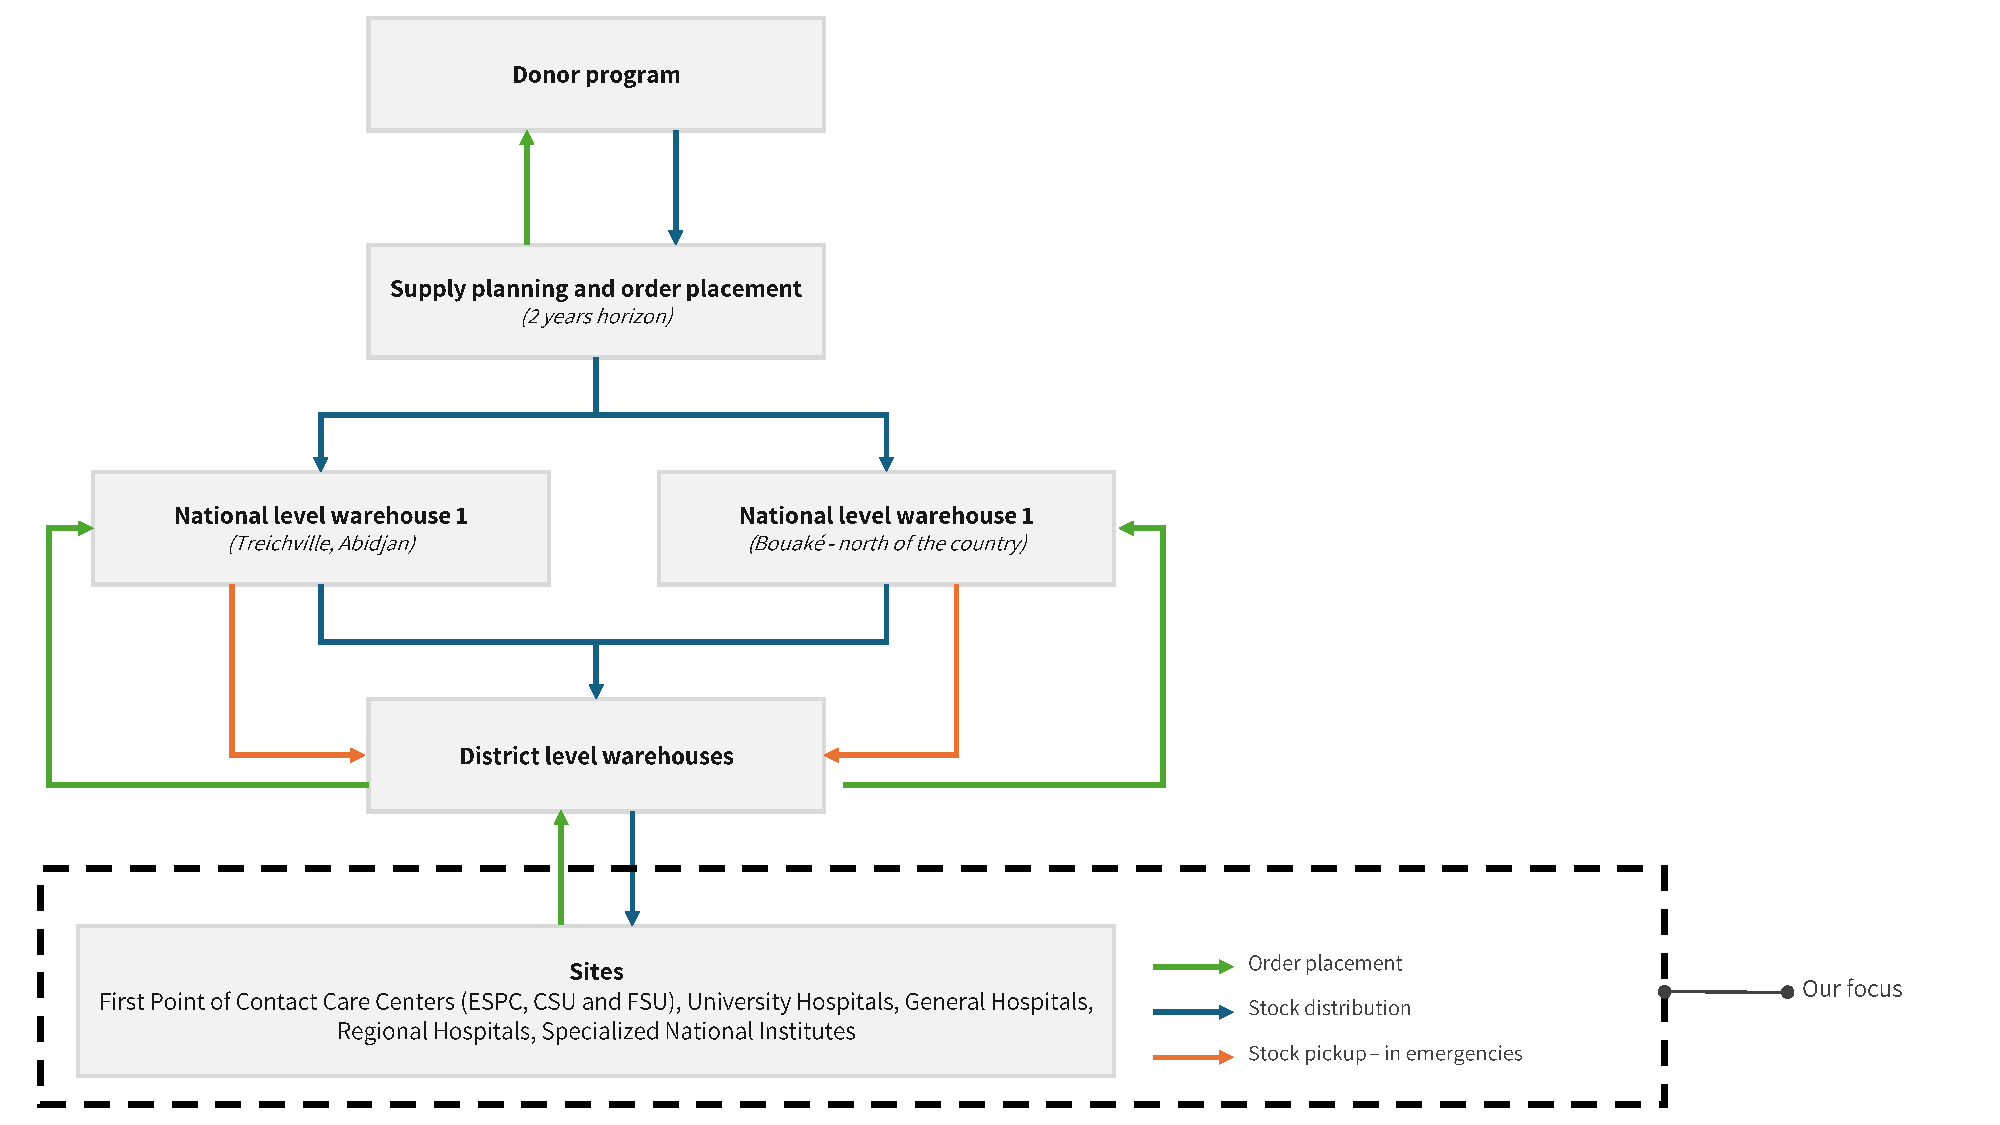
\includegraphics[width=1\linewidth,height=\textheight,keepaspectratio]{E-companion-Figure-01.pdf}

}

\caption{\label{fig-sc_flow}Highlevel family planning supply chain map
of Cote d'Ivoire.}

\end{figure}%

\pagebreak

\subsection{Section 4: Inventory policy}\label{sec-appendix_wp2_3}

\subsubsection{Inventory system and
timing}\label{inventory-system-and-timing}

We simulate a \emph{monthly periodic-review} inventory system with
\emph{lost sales} and a fixed \emph{lead time of one month} (\(L=1\)),
consistent with the replenishment cycle in Côte d'Ivoire. At the end of
each month \(t\), after demand is realised, a facility places an order
\(q_t \ge 0\) that becomes available at the start of month \(t+1\),
where \(q_t\) denotes the order placed at the end of month \(t\) and
received at the start of month \(t+1\).

Let \(I_t\) denote the \emph{on-hand inventory} at the ordering cycle
(end of month \(t\)), and let \(D_t\) denote the (latent) demand
realised during month \(t\). Sales are constrained by availability, and
any unmet demand is treated as lost sales:

\begin{equation}\phantomsection\label{eq-st}{
S_t = \min(I_t, D_t),
\qquad
L_t = D_t - S_t
}\end{equation} Inventory evolves according to:

\begin{equation}\phantomsection\label{eq-it}{
I_{t+1} = I_t - S_t + q_t
}\end{equation}

Ordering decisions are based on the \emph{inventory position}, defined
as on-hand inventory plus pipeline stock. With \(L=1\), pipeline stock
at the end of month \(t\) equals the order placed in the previous month.
Here, \(I_t\) denotes the on-hand inventory at the beginning of period
\(t\), before the order placed in the previous period is received. The
order \(q_{t-1}\) becomes available for use during period \(t\).
Therefore, the inventory available at the beginning of period:

\begin{equation}\phantomsection\label{eq-ip}{
IP_t = I_t + q_{t-1}
}\end{equation}

All replenishment policies considered in this study follow an
order-up-to structure, differing only in how the target level \(U_t\) is
determined. Given a target \(U_t\), the order quantity is:

\begin{equation}\phantomsection\label{eq-qp}{
q_t = \max{0, U_t - IP_t}
}\end{equation}

Contraceptive products are \emph{programmed medicines} predominantly
funded through donor support. As such, facilities typically receive what
they order, and explicit \emph{ordering costs are not a primary concern}
at the facility level. The policies below therefore focus on buffering
demand uncertainty and avoiding stockouts under lost-sales dynamics,
while remaining consistent with observed ordering practice.

\subsubsection{Policy 1: as-is order-up-to policy (current
practice)}\label{policy-1-as-is-order-up-to-policy-current-practice}

The first policy replicates the replenishment logic commonly used in
Côte d'Ivoire's LMIS practice. Facilities compute an average monthly
consumption and maintain a buffer equivalent to three months of demand.
Let \(\hat{D}_t\) denote a point forecast for month \(t+1\) (in
practice, typically derived from recent average consumption). The target
stock level is computed as:

\begin{equation}\phantomsection\label{eq-stock}{
U_t^{(1)} = 3 \times \hat{D}_t
}\end{equation}

The corresponding order quantity is:

\begin{equation}\phantomsection\label{eq-order}{
q_t^{(1)} = \max{0, U_t^{(1)} - IP_t}
}\end{equation}

This as-is policy provides a realistic baseline aligned with current
ordering practice at the facility level.

\subsubsection{Policy 2: quantile-based order-up-to level
(uncertainty-aware
base-stock)}\label{policy-2-quantile-based-order-up-to-level-uncertainty-aware-base-stock}

In FPSC settings, demand is inherently uncertain due to factors such as
reporting delays, irregular ordering behaviours, and intermittent
service disruptions \citep{hewage2025}. Underestimating demand can
result in severe stockouts, directly affecting contraceptive
availability and user satisfaction \citep{karimi2021}. To buffer against
this uncertainty, we enhance the as-is policy by incorporating
\emph{forecast uncertainty} from the forecast distribution.

Instead of targeting the mean or a single point forecast, the
order-up-to level is set using an upper quantile of the forecast
distribution. Let \(Q^{(\alpha)}_t\) denote the \(\alpha\)-level
quantile of the predictive distribution of demand over the lead time
(here one month), obtained using conformal prediction. The target stock
level becomes:

\begin{equation}\phantomsection\label{eq-quantile}{
U_t^{(2)} = Q^{(\alpha)}_t
}\end{equation}

The resulting order quantity is:

\begin{equation}\phantomsection\label{eq-order_qnt}{
q_t^{(2)} = \max{0, U_t^{(2)} - IP_t}
}\end{equation}

We evaluate this policy across several quantile levels
(\(\alpha = 0.80, 0.85, 0.90, 0.95\)), which correspond to different
implicit service-level targets. This allows us to assess how
conservatively facilities must buffer stock to mitigate demand risk.

\subsubsection{Policy 3: myopic lost-sales
policy}\label{policy-3-myopic-lost-sales-policy}

To benchmark against heuristics designed for \emph{lost-sales} systems,
we include a myopic (one-period) policy that selects the order-up-to
target by balancing inventory holding against the consequences of a
stockout in the next period \citep{bijvank2011, zipkin2008}. Let \(h\)
denote a per-unit holding penalty for carrying one unit of inventory for
one month, and let \(p\) denote a per-unit penalty for a lost sale.
Under a one-period approximation, the cost-balanced target corresponds
to the critical fractile:

\begin{equation}\phantomsection\label{eq-ut3}{
U_t^{(3)} = F_t^{-1}\!\left(\frac{p}{p+h}\right)
}\end{equation}

\begin{equation}\phantomsection\label{eq-qt3}{
q_t^{(3)} = \max\{0,\ U_t^{(3)} - IP_t\}
}\end{equation}

where \(F_t\) is the predictive CDF of lead-time demand (here one
month). In implementation, we approximate \(F_t\) using the predictive
distribution implied by conformal prediction, so the target is obtained
as a quantile of the forecast distribution.

Facility-level monetary cost parameters are not available in our
setting. We therefore implement this benchmark using \emph{normalized}
penalty-to-holding ratios \(\kappa = p/h\), which determine the ordering
fractile via \(\alpha = \kappa/(1+\kappa)\). Motivated by the
service-critical nature of contraceptive availability, we consider a
small grid \(\kappa \in \{5,10,20\}\), corresponding to
\(\alpha \in \{0.83, 0.91, 0.95\}\). This provides a transparent
lost-sales benchmark that reflects different degrees of stockout
aversion while remaining comparable across products and facilities.

\subsubsection{Policy 4: oracle benchmark policy (upper
bound)}\label{policy-4-oracle-benchmark-policy-upper-bound}

To provide an upper bound on achievable inventory performance under the
same lead time and lost-sales dynamics, we include an \emph{oracle}
benchmark. The oracle is not implementable in practice; rather, it
provides a best-case reference that has access to information
unavailable to decision makers \citep{sachs2014}.

We consider an oracle that has access to the \emph{latent (true) demand}
process \(D_t^*\). Under \(L=1\), a simple and transparent oracle target
is the next-period latent demand:

\begin{equation}\phantomsection\label{eq-ut5}{
U_t^{(5)} = D_{t+1}^*,
\qquad
q_t^{(5)} = \max{0, U_t^{(5)} - IP_t}
}\end{equation}

This oracle benchmark provides a ceiling on performance and allows us to
quantify how close forecast-driven policies come to a best-case ordering
rule under perfect demand information.

\subsubsection{Experimental framework}\label{experimental-framework}

\begin{figure}[!ht]
\centering
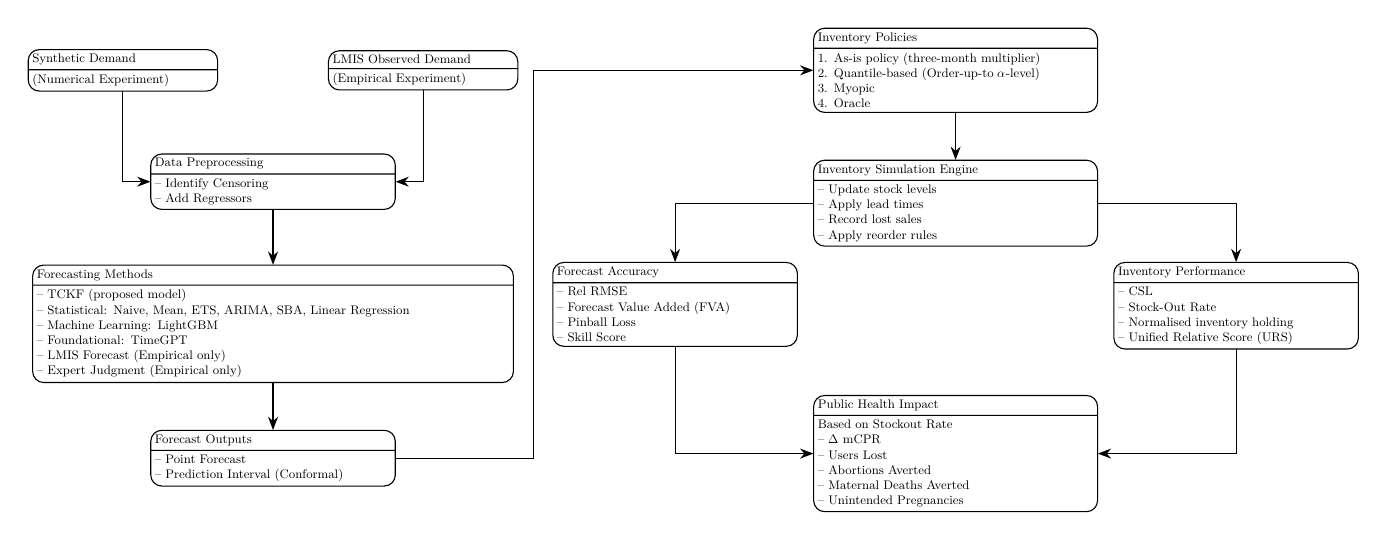
\begin{tikzpicture}[
  scale=0.5, transform shape,
  node distance = 8mm and 10mm,
  >=Stealth,
  every node/.style={font=\small},
  splitbox/.style = {
    rectangle split,
    rectangle split parts=2,
    draw,
    rounded corners,
    align=left,
    inner sep=3pt,
    text width=46mm,
    minimum height=10mm
  },
  splitwide/.style = {
    rectangle split,
    rectangle split parts=2,
    draw,
    rounded corners,
    align=left,
    inner sep=3pt,
    text width=120mm
  },
  splitmid/.style = {
    rectangle split,
    rectangle split parts=2,
    draw,
    rounded corners,
    align=left,
    inner sep=3pt,
    text width=60mm
  },
  splitlong/.style = {
    rectangle split,
    rectangle split parts=2,
    draw,
    rounded corners,
    align=left,
    inner sep=3pt,
    text width=70mm
  }
]

% Top inputs
\node[splitbox] (syn) {
  \textbf{Synthetic Demand}
  \nodepart{second}
  (Numerical Experiment)
};

\node[splitbox, right=28mm of syn] (lmis) {
  \textbf{LMIS Observed Demand}
  \nodepart{second}
  (Empirical Experiment)
};

% Preprocessing
\coordinate (mid) at ($(syn.south)!0.5!(lmis.south)$);
\node[splitmid, below=16mm of mid] (pre) {
  \textbf{Data Preprocessing}
  \nodepart{second}
  -- Identify Censoring\\
  -- Add Regressors
};

% Forecasting methods
\node[splitwide, below=14mm of pre] (fm) {
  \textbf{Forecasting Methods}
  \nodepart{second}
  -- \textbf{TCKF} (proposed model)\\
  -- \emph{Statistical:} Naive, Mean, ETS, ARIMA, SBA, Linear Regression\\
  -- \emph{Machine Learning:} LightGBM\\
  -- \emph{Foundational:} TimeGPT\\
  -- LMIS Forecast (Empirical only)\\
  -- Expert Judgment (Empirical only)
};

% Forecast outputs
\node[splitmid, below=12mm of fm] (fo) {
  \textbf{Forecast Outputs}
  \nodepart{second}
  -- Point Forecast\\
  -- Prediction Interval (Conformal)
};

% Inventory policies
\node[splitlong, right=75mm of lmis] (pol) {
  \textbf{Inventory Policies}
  \nodepart{second}
  1. As-is policy (three-month multiplier)\\
  2. Quantile-based (Order-up-to $\alpha$-level)\\
  3. Myopic\\
  4. Oracle
};

% Simulation engine
\node[splitlong, below=12mm of pol] (sim) {
  \textbf{Inventory Simulation Engine}
  \nodepart{second}
  -- Update stock levels\\
  -- Apply lead times\\
  -- Record lost sales\\
  -- Apply reorder rules
};

% Metrics
\node[splitmid, below left=4mm and 4mm of sim] (fa) {
  \textbf{Forecast Accuracy}
  \nodepart{second}
  -- Rel RMSE\\
  -- Forecast Value Added (FVA)\\
  -- Pinball Loss\\
  -- Skill Score
};

\node[splitmid, below right=4mm and 4mm of sim] (ip) {
  \textbf{Inventory Performance}
  \nodepart{second}
  -- CSL\\
  -- Stock-Out Rate\\
  -- Normalised inventory holding\\
  -- Unified Relative Score (URS)
};

% Public health impact
\coordinate (bottommid) at ($(fa.south)!0.5!(ip.south)$);
\node[splitlong, below=12mm of bottommid] (phi) {
  \textbf{Public Health Impact}
  \nodepart{second}
  Based on Stockout Rate\\
  -- $\Delta$ mCPR\\
  -- Users Lost\\
  -- Abortions Averted\\
  -- Maternal Deaths Averted\\
  -- Unintended Pregnancies
};

% Arrows
\draw[->] (syn.south) |- (pre.west);
\draw[->] (lmis.south) |- (pre.east);
\draw[->] (pre.south) -- (fm.north);
\draw[->] (fm.south)  -- (fo.north);
\path (fo.east) -- +(3.5,0) coordinate (s3stub);
\draw[->] (fo.east) -- (s3stub) |- (pol.west);
\draw[->] (pol.south) -- (sim.north);
\draw[->] (sim.west) -| (fa.north);
\draw[->] (sim.east) -| (ip.north);
\draw[->] (fa.south) |- (phi.west);
\draw[->] (ip.south) |- (phi.east);

\end{tikzpicture}
\caption{Overview of the experimental framework for evaluating contraceptive demand forecasts under censoring.}
\label{fig:conceptual-framework}
\end{figure}

\subsubsection{Lead-time sensitivity
design}\label{lead-time-sensitivity-design}

To check this assumption, we used the stock movement data to construct
an approximate lead-time proxy. For each case where an order was placed
and stock was later received, we calculated the number of months between
the order and the next recorded stock receipt. We also cross-checked
these patterns against demand planner comments, particularly comments
referring to delayed deliveries, pending orders, stock not received,
upstream stockouts, or late shipments. The median delay was one month
and the mean delay was 1.97 months. Around \(54.7\%\) of receipts
occurred within one month, \(16.2\%\) after two months, and \(23.2\%\)
after three or more months. Cases where no later stock receipt was
observed were treated as incomplete and were not used to derive the
stochastic lead-time probabilities.

Based on this, we run a lead-time sensitivity analysis with fixed lead
times of \(L=1\), \(L=2\), and \(L=3\), and a stochastic lead-time
setting. For the stochastic setting, we sample from the empirical
distribution after grouping delays into three categories: within one
month as \(L=1\), two months as \(L=2\), and three or more months as
\(L=3\). This gives approximately \(P(L=1)=0.58\), \(P(L=2)=0.17\), and
\(P(L=3)=0.25\). The same sampled lead-time path is used across all
methods and policies within each replication, so that all methods are
evaluated under the same realised supply conditions.

\pagebreak

\pagebreak

\subsection{Section 5: Performance metrics}\label{sec-appendix_wp2_4}

\subsubsection{Forecast metrics}\label{forecast-metrics}

To evaluate the performance of the benchmark forecasting methods in a
way that is both interpretable and operationally meaningful, we use
relative metrics for point forecasts and skill scores for probabilistic
forecasts. This approach allows us to compare each model against the
proposed TCKF benchmark while remaining robust to scale differences
across series.

For point forecasts, we use the \emph{Relative Root Mean Squared Error
(Rel RMSE)}, which quantifies how much better or worse a method performs
relative to TCKF:

\begin{equation}\phantomsection\label{eq-relrmse}{
Rel\ RMSE = \frac{RMSE_{\text{Method}}}{RMSE_{\text{TCKF}}}
}\end{equation}

Values below 1 indicate better performance than TCKF, while values above
1 indicate worse performance \citep{davydenko2013}. The RMSE is defined
as:

\begin{equation}\phantomsection\label{eq-rmse}{
RMSE = \sqrt{\frac{1}{n} \sum_{t=1}^{n} (\hat{y}_t - y_t)^2}
}\end{equation}

where \(\hat{y}_t\) is the forecast and \(y_t\) is the actual observed
value \citep{hyndman2021forecasting}.

To make this more interpretable, we convert Rel RMSE into a
\emph{Forecast Value Added (FVA)} score \citep{gilliland2008fva}:

\begin{equation}\phantomsection\label{eq-fva_1}{
FVA = (1 - Rel\ RMSE) \times 100\%
}\end{equation}

For interval forecasts, we use \emph{Pinball Loss}, which is
particularly suited for evaluating prediction intervals. In FPSC
settings, where service levels are critical, this scoring rule penalises
both \emph{underprediction} and \emph{overprediction} asymmetrically,
making it well-aligned with our goal of reliable and calibrated
uncertainty estimates \citep{kolassa2023}.

The pinball loss at time \(t\) for quantile level \(p\) is defined as:

\begin{equation}\phantomsection\label{eq-pinball}{
Q_{p,t} =
\begin{cases}
2(1 - p)(\hat{f}_{p,t} - y_t), & \text{if } y_t < \hat{f}_{p,t} \\
2p(y_t - \hat{f}_{p,t}), & \text{if } y_t \geq \hat{f}_{p,t}
\end{cases}
}\end{equation}

where \(\hat{f}_{p,t}\) is the predicted quantile at level \(p\), and
\(y_t\) is the actual observed value. Lower values indicate sharper,
better-calibrated intervals \citep{hyndman2021forecasting}.

To assess improvements relative to TCKF, we use the \emph{Pinball Loss
Skill Score} \citep{hyndman2021forecasting}:

\begin{equation}\phantomsection\label{eq-skill}{
\text{Skill Score} = \frac{\text{Pinball Score}_{\text{TCKF}} - \text{Pinball Score}_{\text{Method}}}{\text{Pinball Score}_{\text{TCKF}}} \times 100\%
}\end{equation}

\subsubsection{Price proxies for empirical
data}\label{price-proxies-for-empirical-data}

\begingroup\fontsize{8}{10}\selectfont

\begin{longtable}[t]{>{\raggedright\arraybackslash}p{7em}>{\raggedright\arraybackslash}p{14em}>{\raggedright\arraybackslash}p{8em}}

\caption{\label{tbl-emp-price}Price proxies for empirical data.}

\tabularnewline

\toprule
Product code & Product & Proxy unit price (USD)\\
\midrule
\endfirsthead
\multicolumn{3}{@{}l}{\textit{(continued)}}\\
\toprule
Product code & Product & Proxy unit price (USD)\\
\midrule
\endhead

\endfoot
\bottomrule
\endlastfoot
AS27000 & Microgynon / pill & 0.220\\
AS27132 & Microlut & 0.288\\
AS27133 & Depo Provera injectable & 0.637\\
AS27134 & Noristerat injectable & 0.637\\
AS27138 & Implanon & 10.500\\
\addlinespace
AS27137 & Jadelle & 8.520\\
AS42018 & Copper T IUD & 0.393\\
AS46000 & Male condom & 0.030\\
AS17005 & Female condom & 0.490\\*

\end{longtable}

\endgroup{}

\subsubsection{Public health indicators}\label{public-health-indicators}

In FPSC, a shortage of contraceptives does not merely disrupt service
delivery; it directly contributes to avoidable pregnancies, maternal and
infant complications, and lost opportunities for system-wide impact
\citep{karimi2021}. To quantify this, we adopt a public health impact
framework adapted from the RH Supplies Impact Calculator\footnote{RHSC
  Impact Calculator:
  \url{https://www.rhsupplies.org/activities-resources/tools/reducing-stockouts-impact-calculator}}.
This model links changes in contraceptive availability to shifts in
modern contraceptive prevalence rate (mCPR)\footnote{Percentage of women
  of reproductive age using modern contraceptive methods.}, drawing on
empirical estimates from \citet{karim2008measuring},
\citet{wang_how_2012}, and \citet{ross2012use}. Based on these studies,
\citet{rosen2018modeling} estimate that the addition of one method can
increase mCPR by 6.5 percentage points.

Under the RHSC logic, reducing stockouts increases method availability,
which in turn raises contraceptive use. We therefore express the change
in mCPR relative to the TCKF benchmark as:

\begin{equation}\phantomsection\label{eq-mcrp}{
\Delta mCPR = 0.065 \times M \times (SOR_{\text{TCKF}} - SOR_{\text{Method}}),
}\end{equation}

where \(M\) is the number of distinct methods considered. The
corresponding change in users is:

\begin{equation}\phantomsection\label{eq-ul}{
\text{Users Gained} = \Delta mCPR \times \text{WRA Population},
}\end{equation}

where \(\text{WRA Population}\) is the number of women of reproductive
age. To estimate downstream outcomes, we apply conversion factors from
the Adding It Up study \citep{Singh2009}:

\begin{itemize}
\tightlist
\item
  Maternal deaths averted: \(\frac{\text{Users Gained}}{3153}\)
\item
  Infant deaths averted: \(\frac{\text{Users Gained}}{251}\)
\item
  Abortions averted: \(\frac{\text{Users Gained}}{6.46}\)
\item
  Unintended pregnancies averted: \(\frac{\text{Users Gained}}{3.63}\)
\end{itemize}

\subsubsection{Inventory metrics and relative mCPR
loss}\label{inventory-metrics-and-relative-mcpr-loss}

In addition to forecast accuracy, we evaluate whether the forecasts lead
to better inventory decisions. We focus on the trade-off between product
availability, unmet demand, and inventory burden.

In the numerical experiment, true demand is known. Therefore, we
calculate achieved CSL as the proportion of periods where opening stock
is sufficient to meet demand:

\begin{equation}\phantomsection\label{eq-csl}{
CSL = \frac{1}{N}\sum_{i,t} \mathbb{I}\left(S_{i,t}^{open} \geq D_{i,t}\right)
}\end{equation}

where \(D_{i,t}\) is the true demand and \(S_{i,t}^{open}\) is the
opening stock. We also calculate lost demand as

\begin{equation}\phantomsection\label{eq-ld}{
L_{i,t} = \max(D_{i,t} - S_{i,t}^{open},0)
}\end{equation}

and report the lost-demand rate as

\begin{equation}\phantomsection\label{eq-ldr}{
LDR = \frac{\sum_{i,t} L_{i,t}}{\sum_{i,t} D_{i,t}}
}\end{equation}

Inventory burden is measured using average opening inventory:

\begin{equation}\phantomsection\label{eq-avg_inv}{
\bar{S}^{open} = \frac{1}{N}\sum_{i,t} S_{i,t}^{open}
}\end{equation}

In the empirical experiment, true demand is not observed during
stockouts and service interruptions. Therefore, the simulated inventory
evaluation is calculated over uncensored observations, where recorded
stock distributed is treated as observed demand. We report achieved CSL,
lost-demand rate, and opening months of stock (MOS). Opening MOS is
calculated as

\begin{equation}\phantomsection\label{eq-mos}{
MOS^{open}_{m,p} =
\frac{\sum_{j,s,t} S_{j,s,t}^{open}}
{\sum_{j,s,t} D_{j,s,t}}
}\end{equation}

where \(D_{j,s,t}\) is observed demand for product \(j\), site \(s\),
and month \(t\), and \(S_{j,s,t}^{open}\) is opening stock.

To capture the financial burden of overstocking, we also calculate total
opening inventory value in the empirical experiment. Since item-level
procurement prices were not available in the LMIS dataset, we use
product-level proxy unit prices. These proxy prices were obtained from
publicly available USAID reference price information
\citep{rosen2018modeling} where a close product match was available, and
were cross-checked through discussions with pharmaceutical supply chain
practitioners in Ethiopia. Therefore, they should be interpreted as
approximate valuation inputs rather than official procurement costs for
Côte d'Ivoire. The proxy prices are reported above. Let \(c_j\) denote
the proxy unit price for product \(j\). Then,

\begin{equation}\phantomsection\label{eq-inv_val}{
V^{open}_{m,p} =
\sum_{j,s,t} c_j S_{j,s,t}^{open}
}\end{equation}

\paragraph{Public health indicators}\label{public-health-indicators-1}

Beyond operational inventory metrics, we assess how stockouts translate
into missed public health outcomes. We adopt a public health impact
framework adapted from the RH Supplies Impact Calculator\footnote{RHSC
  Impact Calculator:
  \url{https://www.rhsupplies.org/activities-resources/tools/reducing-stockouts-impact-calculator}}
to link stockout rates to changes in mCPR and downstream outcomes (Users
Lost, Unintended Pregnancies, etc.).

We use stockout rates for this translation because stockouts represent
interruptions in access. Let \(SO_{m,p}\) denote the stockout rate for
method \(m\) and policy \(p\), and let \(SO_{b,p}\) denote the benchmark
stockout rate under the same policy. The relative stockout difference is

\begin{equation}\phantomsection\label{eq-so}{
\Delta SO_{m,p} = SO_{m,p} - SO_{b,p}
}\end{equation}

Relative mCPR loss is calculated as

\begin{equation}\phantomsection\label{eq-mcpr}{
\Delta mCPR_{m,p} = \rho  \Delta SO_{m,p}
}\end{equation}

where \(\rho = 0.065\) is the assumed mCPR contribution per method
category and \(J\) is the number of contraceptive product categories
included in the empirical analysis. Positive values indicate higher mCPR
loss relative to the benchmark, while negative values indicate lower
relative loss.

While these estimates are illustrative and not facility-specific, they
provide a practical way to interpret stockout outcomes through the lens
of public health. In doing so, we emphasise that inventory performance
is not purely an operational concern but a proxy for real-world health
impact in systems where availability governs access.

\pagebreak

\subsection{Section 6: Synthetic data generation and demand
characteristics}\label{sec-appendix_wp2_5}

\begin{algorithm}[H]
\scriptsize
\SetAlgoNlRelativeSize{-2}
\SetAlCapSkip{0.5em}
\SetInd{0.5em}{1em}
\DontPrintSemicolon
\caption{Synthetic time series generation -- Part 1}
\label{alg:synthetic_generation_part1}

\KwIn{
  $P$ products, $S$ stores, $T$ periods, dates with monthly index; \\
  types $\in \{\textsf{smooth},\textsf{erratic},\textsf{lumpy}\}$; \\
  correlation labels $\in \{\textsf{correlated},\textsf{uncorrelated}\}$; \\
  target STL strengths $(F^{\text{trend}},F^{\text{season}})\in[0,1]^2$; \\
  CV$^2$ targets by type; common-shock weight $\rho \in [0,1]$.
}
\KwOut{Intermediate latent series up to $x^{\text{all}}_t$ for each product--store pair}

\BlankLine
\textbf{Shared structures:} draw a 12-month \textit{shared seasonal} vector and a length-$T$ \textit{common shock}, both centered.\;

\textbf{Parameter grid:} for each product--store pair, assign
(i) \textit{series\_category} $\in$ \{correlated, uncorrelated\},
(ii) \textit{series\_type} $\in$ \{smooth, erratic, lumpy\},
(iii) \textit{trend\_strength} $\in$ \{low, medium, high\},
(iv) \textit{seasonal\_strength} $\in$ \{low, medium, high\}; \\
map these to initial slope and seasonal amplitude ranges.\;

\ForEach{series}{
  \tcp{Seasonal pattern by correlation label}
  \eIf{correlated}{
    use the shared seasonal vector
  }{
    draw a new centered seasonal vector of length 12
  }

  \tcp{Weaken deterministic structure for \textsf{erratic} series}
  \If{type = erratic}{
    scale slope $\leftarrow 0.3\times$, season\_amp $\leftarrow 0.5\times$
  }

  \tcp{Choose CV$^2$ target by type (log-uniform on CV)}
  Set CV$^2$ target: smooth $\sim$ low, erratic $\sim$ medium--high, lumpy $\sim$ medium--very high.\;

  \tcp{Noise-aware calibration: match STL strengths}
  Draw target $(F^{\text{trend}}_{\star},F^{\text{season}}_{\star})$ (e.g., Beta(2,2)); \\
  \For{$k=1$ \KwTo 3}{
    form baseline $b_t = (\text{slope}\cdot t) + (\text{season\_amp}\cdot \text{seas}(t))$;\;
    shift $b_t$ to positive support; \\
    draw multiplicative noise $\varepsilon_t \sim \log\mathcal{N}(\mu,\sigma^2)$ s.t. $E[\varepsilon_t]=1$, $\operatorname{Var}[\varepsilon_t]=$CV$^2$; \\
    compute provisional series $z_t = b_t \cdot \varepsilon_t$; \\
    compute STL strengths $(\widehat{F}^{\text{trend}},\widehat{F}^{\text{season}})$; \\
    update \textit{slope}, \textit{season\_amp} multiplicatively to reduce $(F_\star - \widehat{F})$.
  }

  \tcp{Deterministic component}
  $b_t \leftarrow (\text{slope}\cdot t) + (\text{season\_amp}\cdot \text{seas}(t))$; \\
  shift $b_t$ to positive.\;

  \tcp{Correlated multiplicative shock (common + idiosyncratic)}
  Draw idiosyncratic standardized shock $z^{\text{id}}_t$: \\
  \hspace*{1em} smooth: i.i.d. $\mathcal{N}(0,1)$; \\
  \hspace*{1em} erratic: AR(1) with $\phi \in [0.3,0.6]$; \\
  \hspace*{1em} lumpy: standardized $t_{\nu=3}$.\;
  
  \eIf{correlated}{
    set $z_t \leftarrow \sqrt{\rho}\,z^{\text{common}}_t + \sqrt{1-\rho}\,z^{\text{id}}_t$
  }{
    set $z_t \leftarrow z^{\text{id}}_t$
  }\;

  Convert CV$^2$ target to $\sigma^2 = \log(1+\text{CV}^2)$; \\
  set $\varepsilon_t \leftarrow \exp\{\sigma z_t - \tfrac{1}{2}\sigma^2\}$ so $E[\varepsilon_t]=1$, $\operatorname{Var}=\text{CV}^2$.\;

  \tcp{Multiplicative series and level scaling}
  Form $x^{\text{raw}}_t = b_t \cdot \varepsilon_t$; \\
  draw a desired mean $\bar{x}$ (e.g., Uniform[20,100]); \\
  rescale to $x^{\text{all}}_t = x^{\text{raw}}_t \cdot \bar{x} / \overline{x^{\text{raw}}}$.\;
}
\end{algorithm}

\begin{algorithm}[H]
\scriptsize
\SetAlgoNlRelativeSize{-2}
\SetAlCapSkip{0.5em}
\SetInd{0.5em}{1em}
\DontPrintSemicolon
\caption{Synthetic time series generation -- Part 2}
\label{alg:synthetic_generation_part2}

\KwIn{Intermediate latent series $x^{\text{all}}_t$ for each product--store pair}
\KwOut{Panel dataset with \texttt{actual\_demand}, \texttt{observed\_demand}, \texttt{censoring\_type}}

\ForEach{series}{
  \tcp{Type-dependent spikes and zeros}
  \If{type $\in$ \{erratic, lumpy\}}{
    sample indices and multiply $x^{\text{all}}_t$ by log-normal spike factors (higher freq/size for erratic).
  }
  
  \If{type = lumpy}{
    set $x_t = x^{\text{all}}_t \cdot \mathbb{I}(\text{Bern}(p_{nz}\in[0.3,0.7]))$
  }
  \ElseIf{type = erratic}{
    set $x_t = x^{\text{all}}_t \cdot \mathbb{I}(\text{Bern}(p_{nz}\in[0.8,1.0]))$
  }
  \Else{
    set $x_t = x^{\text{all}}_t$
  }

  \tcp{Block censoring until target proportion is covered}
  Initialize $y_t \leftarrow x_t$, \texttt{censoring\_type}$\leftarrow$ "none"; \\
  draw target censor share $q \sim \text{Uniform}(0.20, 0.40)$ and total censored count $qT$; \\
  sample block lengths $L$ (1 with prob 0.7; otherwise 2--5) until $\sum L \ge qT$; \\
  trim last block; \\
  for each block, sample \textsf{event} $\in \{\textsf{disruption}, \textsf{censored}\}$ with probs (0.3, 0.7) and a start index avoiding overlap.\;

  \eIf{\textsf{event} = disruption}{
    set $y_t = 0$ and tag "disruption"
  }{
    set $y_t = u \cdot x_t$ with $u \sim \text{Uniform}(0.3,0.8)$ and tag "censored"
  }.

  \tcp{Record}
  Save \{date, series\_category, series\_type, store, product, 
  actual\_demand $=x_t$, observed\_demand $=y_t$, censoring\_type\}.
}
\end{algorithm}

\subsubsection{Synthetic and empirical demand
characteristics}\label{synthetic-and-empirical-demand-characteristics}

\begin{figure}[htbp]

\centering{

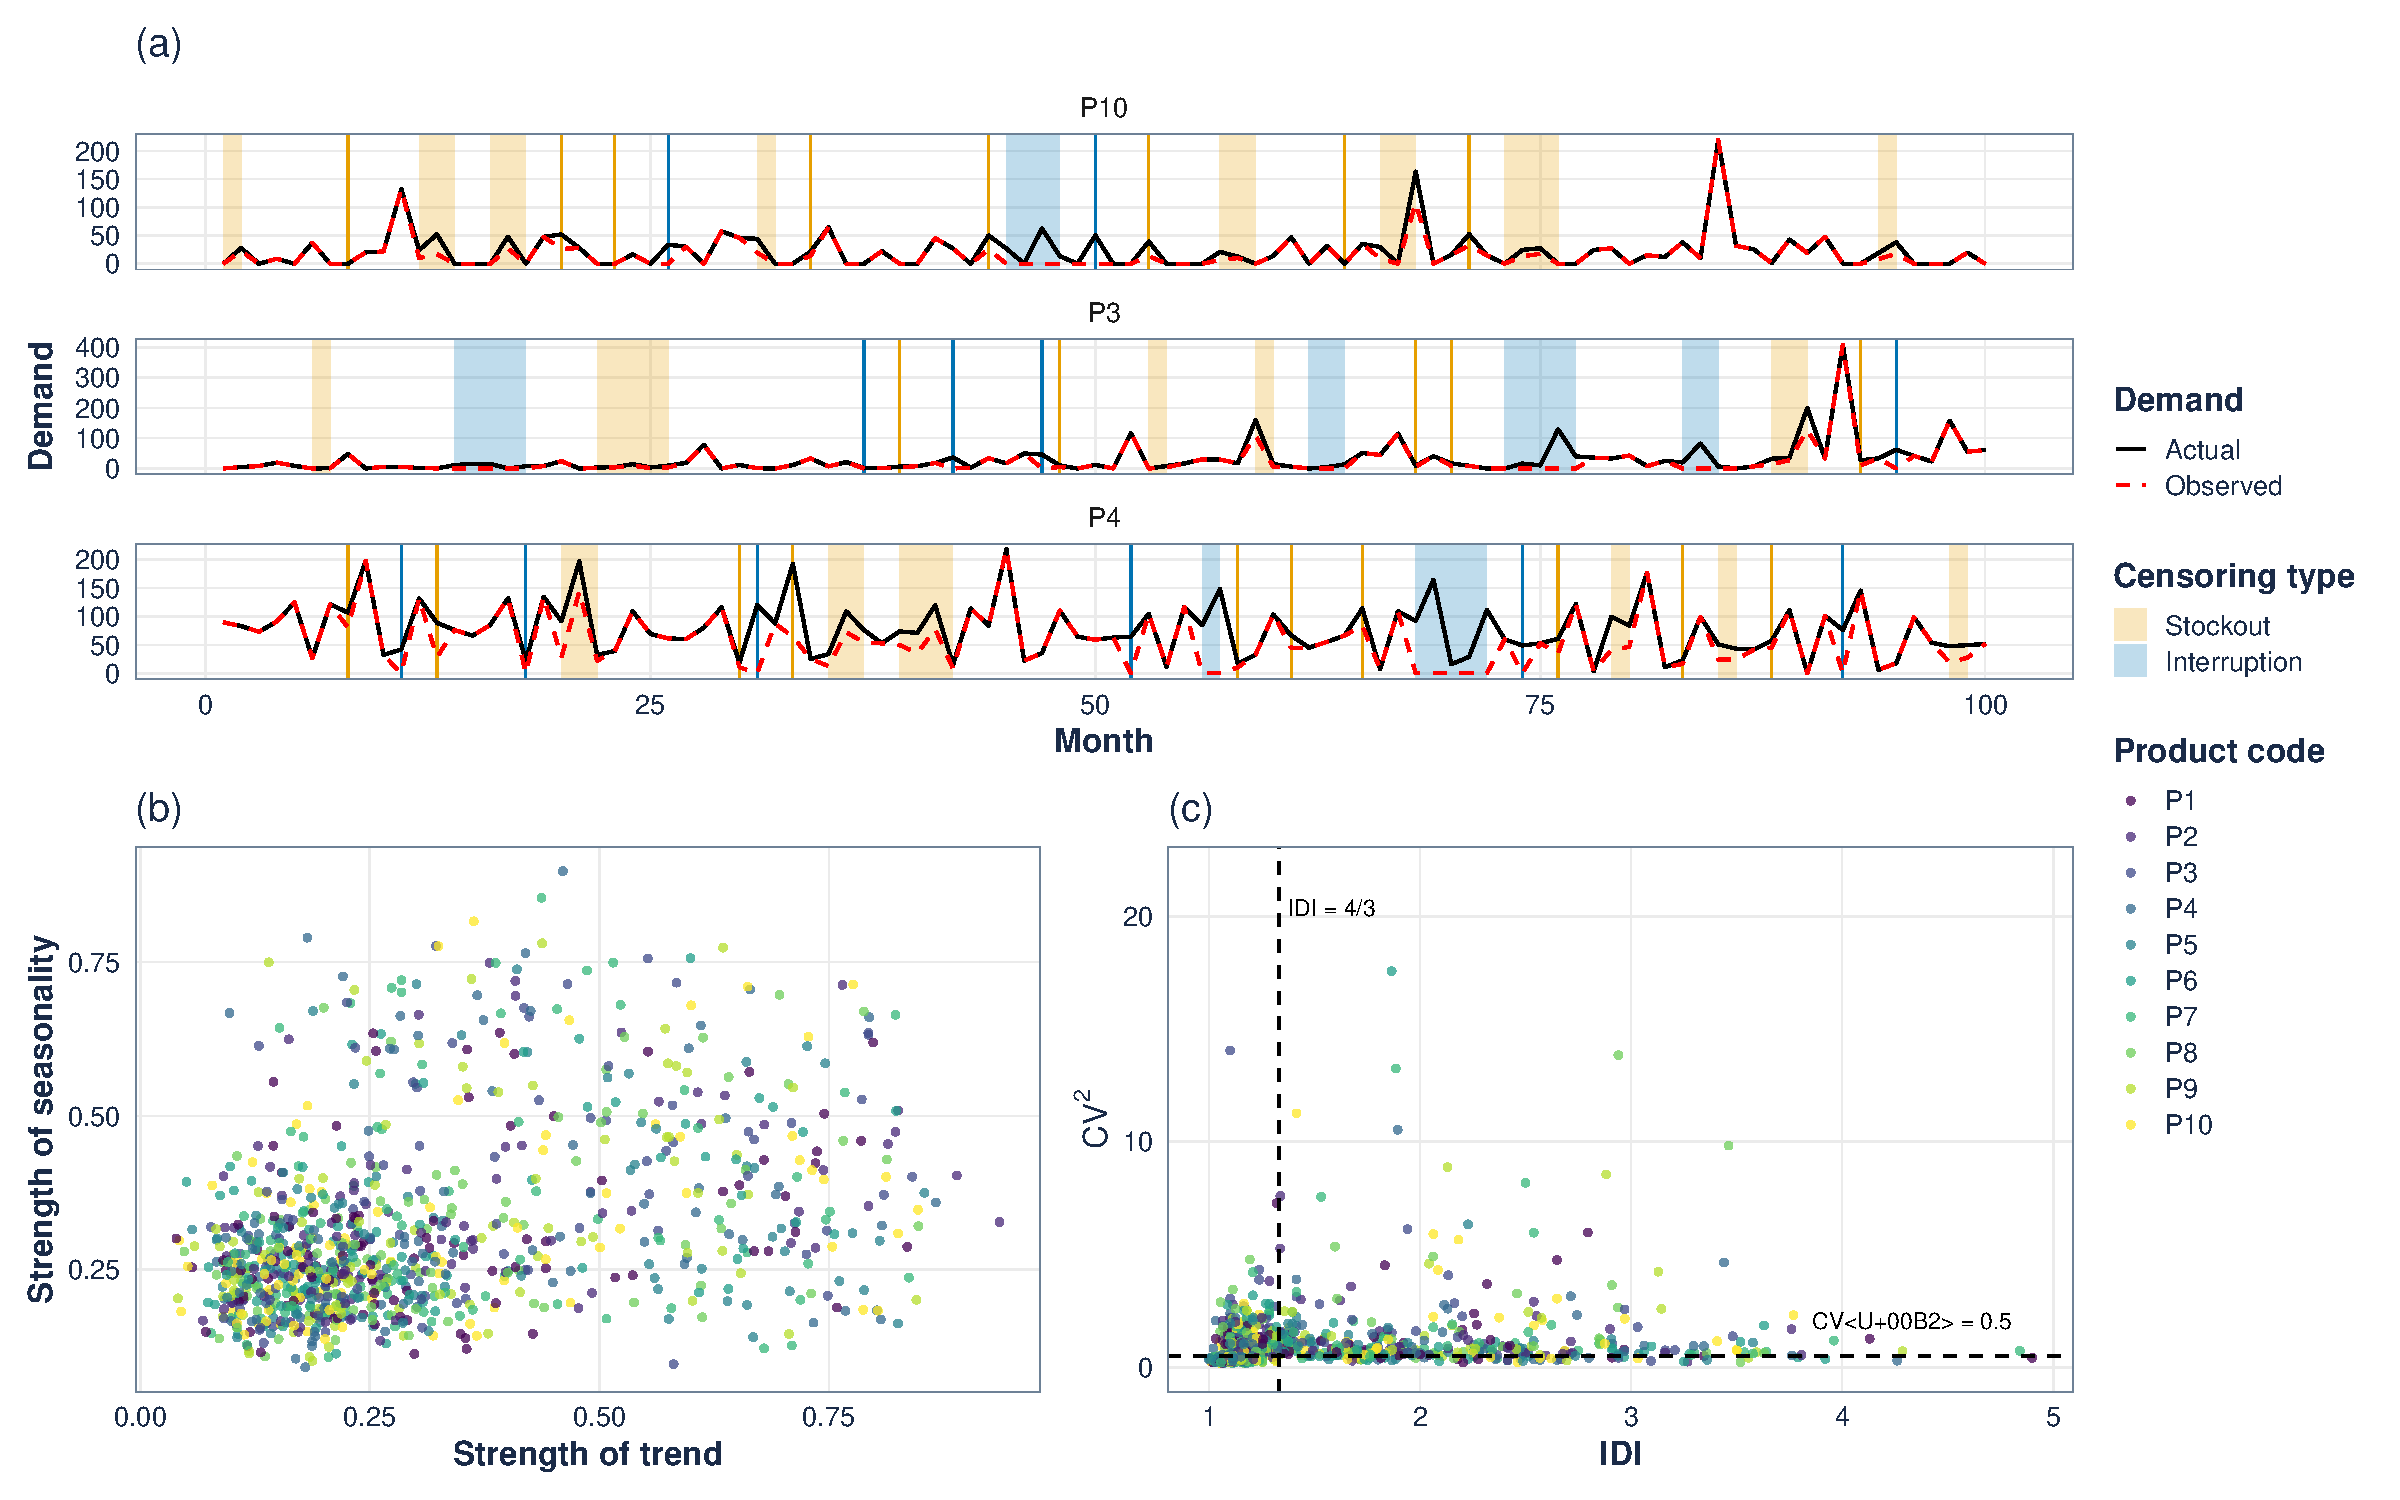
\includegraphics[width=0.75\linewidth,height=\textheight,keepaspectratio]{E-companion-Figure-03.pdf}

}

\caption{\label{fig-ts_feat1_wp2}Time-series characteristics of the
synthetic dataset used in the numerical experiment; (a) Representative
time series; (b) distribution of series by trend and seasonality
strength; (c) intermittency classification using IDI and \(CV^2\)
thresholds.}

\end{figure}%

\begin{figure}

\centering{

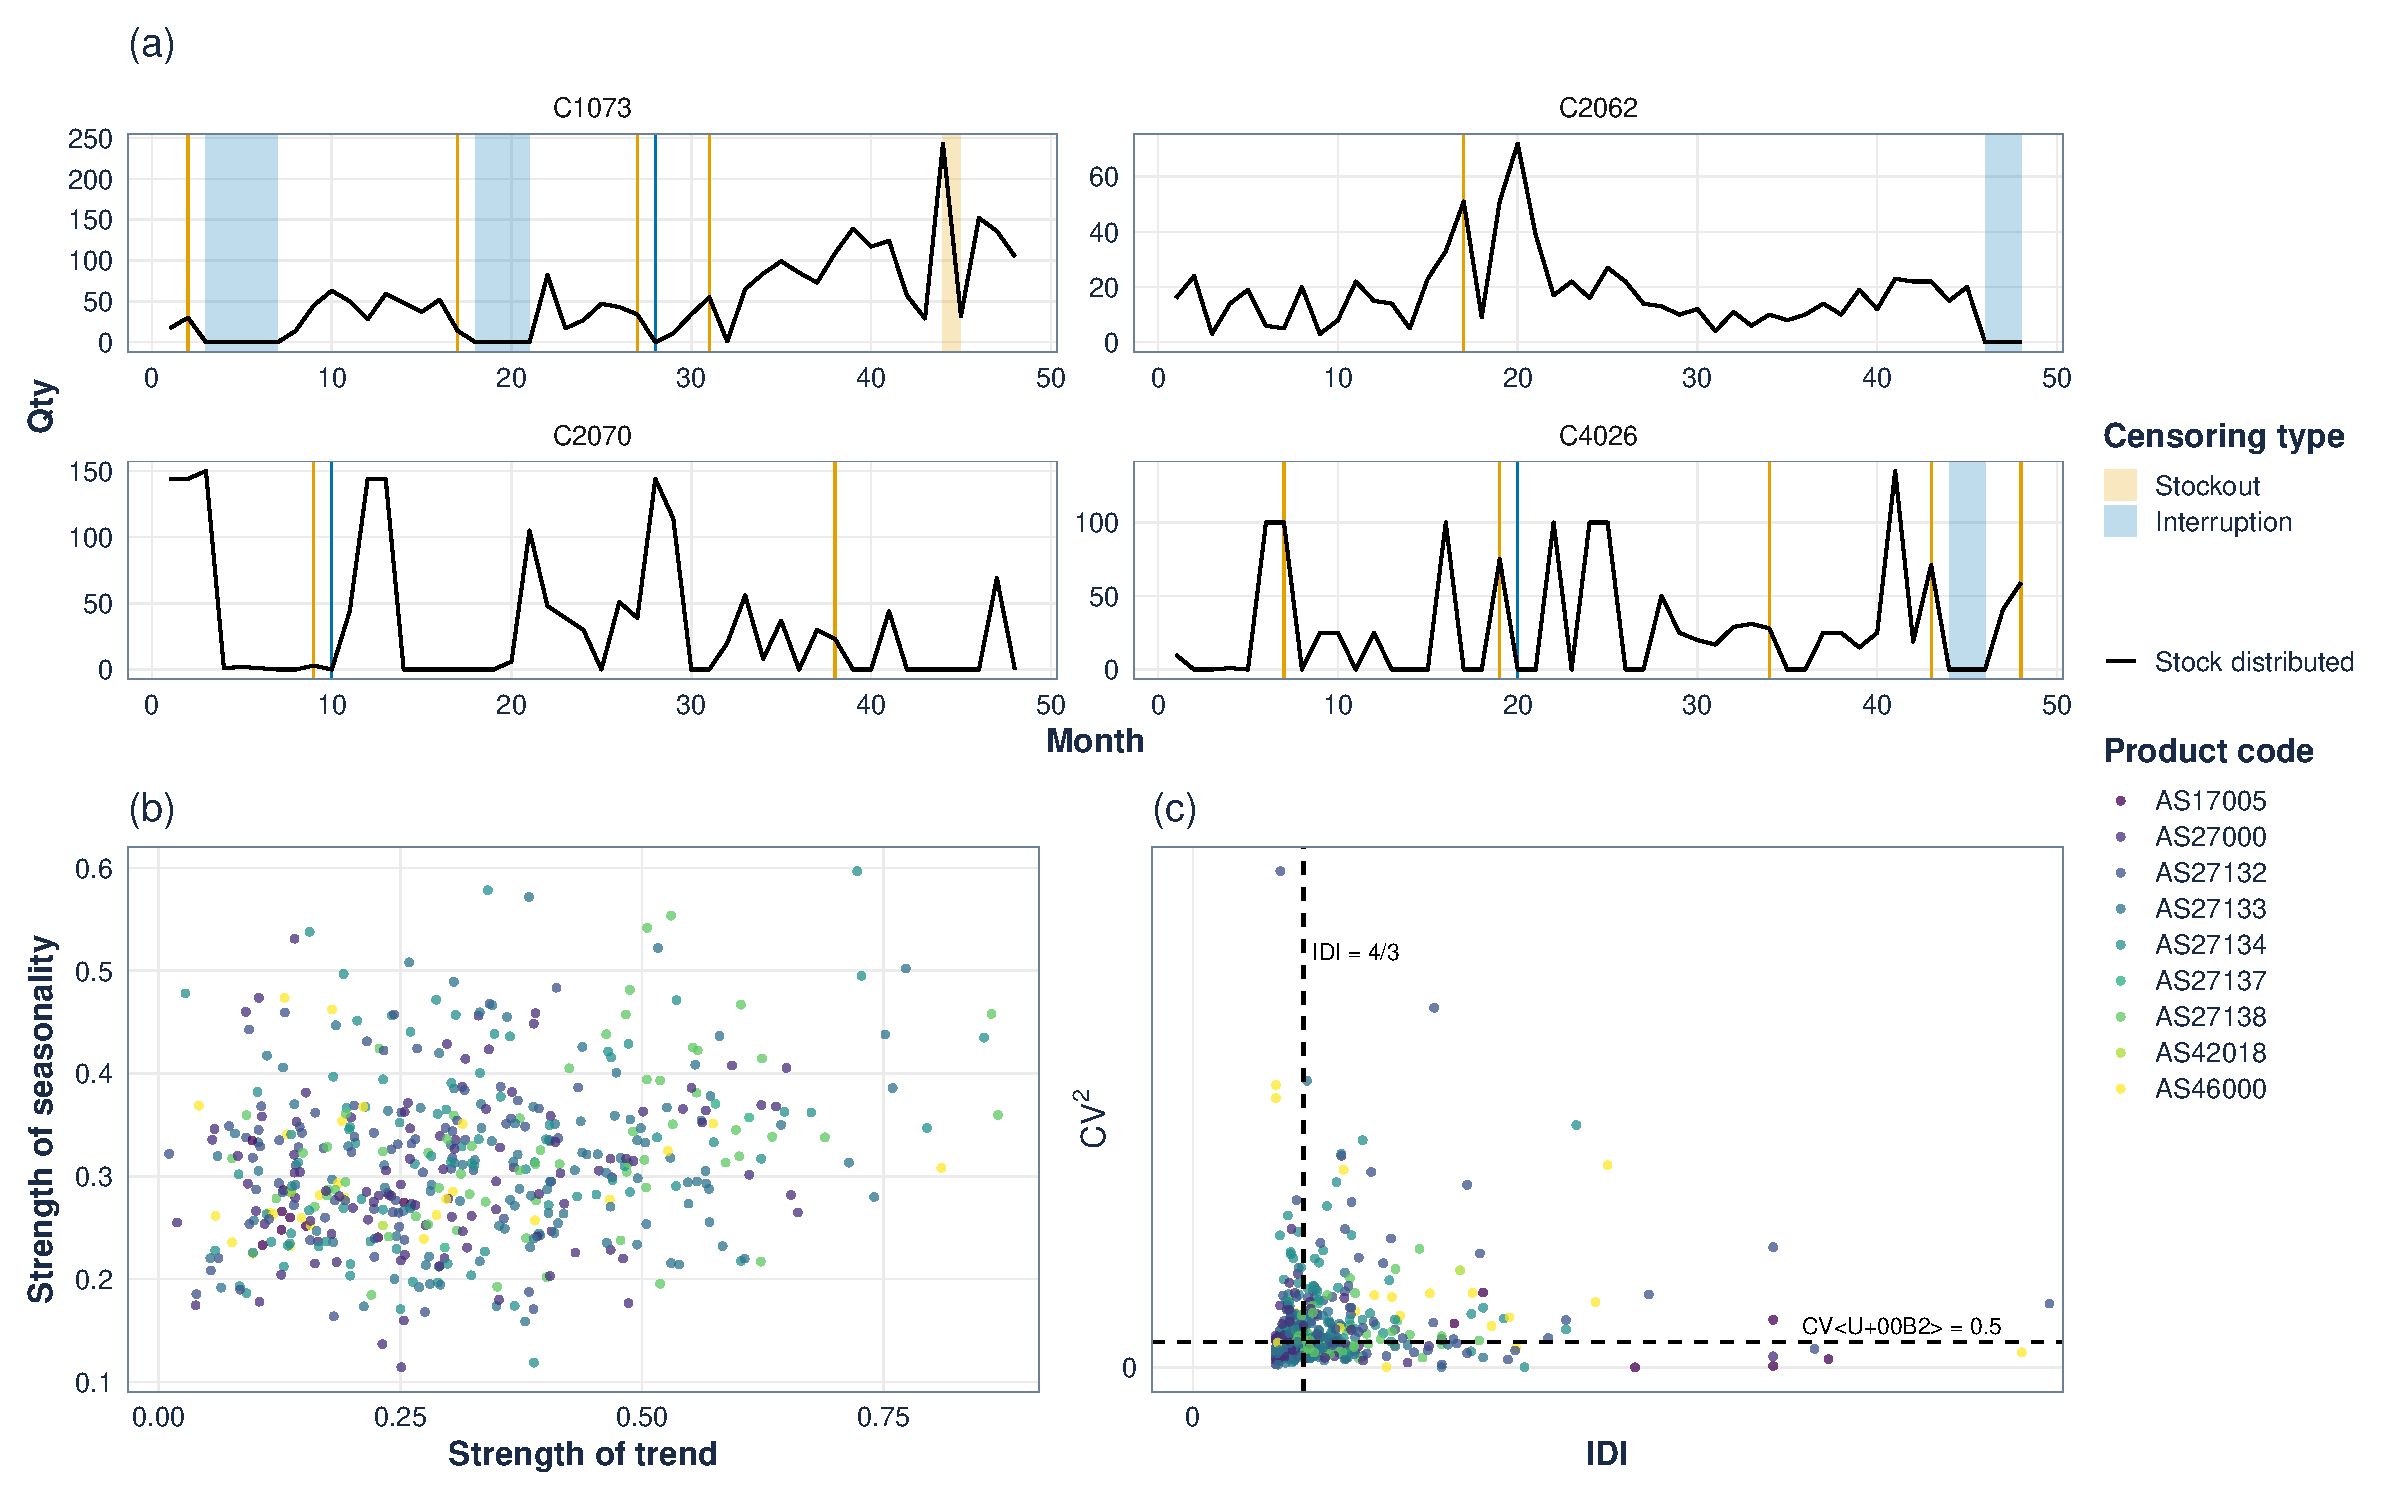
\includegraphics[width=0.75\linewidth,height=\textheight,keepaspectratio]{E-companion-Figure-04.pdf}

}

\caption{\label{fig-ts_feat2_wp2}Time-series characteristics of the
real-world dataset used in the empirical evaluation. (a) Representative
time series for each demand type; (b) Distribution of time series by
trend and seasonality strength and; (c) Intermittency classification
based on IDI and \(CV^2\) thresholds.}

\end{figure}%

\pagebreak

\subsection{Section 7: Inventory performance by forecasting method and
replenishment policy}\label{sec-appendix_wp2_6}

\begingroup\fontsize{8}{10}\selectfont

\begin{longtable}{>{\raggedright\arraybackslash}p{7em}>{\raggedright\arraybackslash}p{12em}>{\raggedleft\arraybackslash}p{5em}>{\raggedleft\arraybackslash}p{5em}>{\raggedleft\arraybackslash}p{5em}}

\caption{\label{tbl-num-inv-detailed}Detailed numerical inventory
performance by forecasting method and replenishment policy.}

\tabularnewline

\toprule
Inventory policy & Method & CSL & Lost-demand rate & Avg. inventory\\
\midrule
\endfirsthead
\multicolumn{5}{@{}l}{\textit{(continued)}}\\
\toprule
Inventory policy & Method & CSL & Lost-demand rate & Avg. inventory\\
\midrule
\endhead

\endfoot
\bottomrule
\endlastfoot
 & TCKF & 0.918 & 0.098 & 181.61\\
\nopagebreak
 & Censored Linear Regression & 0.924 & 0.096 & 183.57\\
\nopagebreak
 & Linear Regression & 0.904 & 0.113 & 158.99\\
\nopagebreak
 & Mean & 0.864 & 0.150 & 158.56\\
\nopagebreak
 & Censored Mean & 0.903 & 0.116 & 182.86\\
\nopagebreak
 & Naive & 0.899 & 0.118 & 262.94\\
\nopagebreak
 & Syntetos-Boylan Approx & 0.885 & 0.134 & 116.81\\
\nopagebreak
 & ARIMA & 0.869 & 0.145 & 129.31\\
\nopagebreak
 & Censored ARIMA & 0.902 & 0.118 & 156.92\\
\nopagebreak
 & ETS & 0.872 & 0.140 & 131.13\\
\nopagebreak
 & TimeGPT & 0.876 & 0.137 & 147.39\\
\nopagebreak
 & Censored TimeGPT & 0.806 & 0.211 & 161.52\\
\nopagebreak
\multirow{-13}{*}{\raggedright\arraybackslash As-is policy} & LightGBM & 0.887 & 0.139 & 117.07\\
\cmidrule{1-5}\pagebreak[0]
 & TCKF & 0.842 & 0.147 & 86.16\\
\nopagebreak
 & Censored Linear Regression & 0.660 & 0.247 & 58.95\\
\nopagebreak
 & Linear Regression & 0.654 & 0.254 & 58.17\\
\nopagebreak
 & Mean & 0.728 & 0.226 & 67.51\\
\nopagebreak
 & Censored Mean & 0.759 & 0.202 & 69.75\\
\nopagebreak
 & Naive & 0.768 & 0.204 & 89.33\\
\nopagebreak
 & Syntetos-Boylan Approx & 0.703 & 0.232 & 54.71\\
\nopagebreak
 & ARIMA & 0.669 & 0.257 & 54.66\\
\nopagebreak
 & Censored ARIMA & 0.659 & 0.255 & 55.10\\
\nopagebreak
 & ETS & 0.659 & 0.261 & 53.73\\
\nopagebreak
 & TimeGPT & 0.737 & 0.212 & 87.09\\
\nopagebreak
 & Censored TimeGPT & 0.682 & 0.325 & 92.76\\
\nopagebreak
\multirow{-13}{*}{\raggedright\arraybackslash Myopic (k=5)} & LightGBM & 0.726 & 0.221 & 59.76\\
\cmidrule{1-5}\pagebreak[0]
 & TCKF & 0.874 & 0.127 & 97.44\\
\nopagebreak
 & Censored Linear Regression & 0.724 & 0.201 & 71.40\\
\nopagebreak
 & Linear Regression & 0.722 & 0.205 & 70.96\\
\nopagebreak
 & Mean & 0.807 & 0.170 & 85.65\\
\nopagebreak
 & Censored Mean & 0.833 & 0.152 & 87.61\\
\nopagebreak
 & Naive & 0.835 & 0.155 & 108.27\\
\nopagebreak
 & Syntetos-Boylan Approx & 0.791 & 0.173 & 71.81\\
\nopagebreak
 & ARIMA & 0.754 & 0.195 & 70.89\\
\nopagebreak
 & Censored ARIMA & 0.736 & 0.197 & 70.60\\
\nopagebreak
 & ETS & 0.742 & 0.201 & 69.61\\
\nopagebreak
 & TimeGPT & 0.761 & 0.195 & 100.39\\
\nopagebreak
 & Censored TimeGPT & 0.713 & 0.296 & 113.75\\
\nopagebreak
\multirow{-13}{*}{\raggedright\arraybackslash Myopic (k=10)} & LightGBM & 0.793 & 0.175 & 73.96\\
\cmidrule{1-5}\pagebreak[0]
 & TCKF & 0.899 & 0.108 & 112.81\\
\nopagebreak
 & Censored Linear Regression & 0.776 & 0.164 & 86.89\\
\nopagebreak
 & Linear Regression & 0.778 & 0.166 & 86.74\\
\nopagebreak
 & Mean & 0.861 & 0.131 & 106.35\\
\nopagebreak
 & Censored Mean & 0.880 & 0.120 & 107.34\\
\nopagebreak
 & Naive & 0.876 & 0.122 & 129.43\\
\nopagebreak
 & Syntetos-Boylan Approx & 0.850 & 0.133 & 91.78\\
\nopagebreak
 & ARIMA & 0.815 & 0.152 & 90.18\\
\nopagebreak
 & Censored ARIMA & 0.793 & 0.156 & 88.85\\
\nopagebreak
 & ETS & 0.801 & 0.158 & 88.68\\
\nopagebreak
 & TimeGPT & 0.773 & 0.187 & 108.43\\
\nopagebreak
 & Censored TimeGPT & 0.729 & 0.282 & 127.07\\
\nopagebreak
\multirow{-13}{*}{\raggedright\arraybackslash Myopic (k=20)} & LightGBM & 0.845 & 0.138 & 91.80\\
\cmidrule{1-5}\pagebreak[0]
 & TCKF & 0.831 & 0.153 & 83.08\\
\nopagebreak
 & Censored Linear Regression & 0.640 & 0.264 & 55.59\\
\nopagebreak
 & Linear Regression & 0.629 & 0.272 & 54.67\\
\nopagebreak
 & Mean & 0.696 & 0.249 & 62.29\\
\nopagebreak
 & Censored Mean & 0.729 & 0.222 & 64.66\\
\nopagebreak
 & Naive & 0.743 & 0.224 & 83.67\\
\nopagebreak
 & Syntetos-Boylan Approx & 0.669 & 0.254 & 49.93\\
\nopagebreak
 & ARIMA & 0.639 & 0.280 & 50.20\\
\nopagebreak
 & Censored ARIMA & 0.632 & 0.276 & 50.85\\
\nopagebreak
 & ETS & 0.630 & 0.284 & 49.32\\
\nopagebreak
 & TimeGPT & 0.726 & 0.220 & 81.57\\
\nopagebreak
 & Censored TimeGPT & 0.667 & 0.340 & 84.72\\
\nopagebreak
\multirow{-13}{*}{\raggedright\arraybackslash Quantile 80} & LightGBM & 0.702 & 0.237 & 56.24\\
\cmidrule{1-5}\pagebreak[0]
 & TCKF & 0.847 & 0.144 & 87.71\\
\nopagebreak
 & Censored Linear Regression & 0.670 & 0.240 & 60.65\\
\nopagebreak
 & Linear Regression & 0.666 & 0.246 & 59.94\\
\nopagebreak
 & Mean & 0.742 & 0.216 & 70.16\\
\nopagebreak
 & Censored Mean & 0.773 & 0.193 & 72.33\\
\nopagebreak
 & Naive & 0.780 & 0.195 & 92.20\\
\nopagebreak
 & Syntetos-Boylan Approx & 0.717 & 0.221 & 57.14\\
\nopagebreak
 & ARIMA & 0.682 & 0.246 & 56.93\\
\nopagebreak
 & Censored ARIMA & 0.672 & 0.245 & 57.26\\
\nopagebreak
 & ETS & 0.673 & 0.251 & 55.98\\
\nopagebreak
 & TimeGPT & 0.743 & 0.208 & 89.93\\
\nopagebreak
 & Censored TimeGPT & 0.689 & 0.318 & 97.08\\
\nopagebreak
\multirow{-13}{*}{\raggedright\arraybackslash Quantile 85} & LightGBM & 0.736 & 0.214 & 61.55\\
\cmidrule{1-5}\pagebreak[0]
 & TCKF & 0.868 & 0.132 & 94.60\\
\nopagebreak
 & Censored Linear Regression & 0.711 & 0.211 & 68.46\\
\nopagebreak
 & Linear Regression & 0.708 & 0.215 & 67.97\\
\nopagebreak
 & Mean & 0.793 & 0.180 & 81.68\\
\nopagebreak
 & Censored Mean & 0.820 & 0.161 & 83.83\\
\nopagebreak
 & Naive & 0.823 & 0.164 & 104.19\\
\nopagebreak
 & Syntetos-Boylan Approx & 0.775 & 0.184 & 68.00\\
\nopagebreak
 & ARIMA & 0.739 & 0.207 & 67.22\\
\nopagebreak
 & Censored ARIMA & 0.721 & 0.208 & 67.14\\
\nopagebreak
 & ETS & 0.726 & 0.212 & 65.99\\
\nopagebreak
 & TimeGPT & 0.758 & 0.197 & 98.74\\
\nopagebreak
 & Censored TimeGPT & 0.710 & 0.299 & 111.06\\
\nopagebreak
\multirow{-13}{*}{\raggedright\arraybackslash Quantile 90} & LightGBM & 0.778 & 0.184 & 70.59\\
\cmidrule{1-5}\pagebreak[0]
 & TCKF & 0.896 & 0.111 & 110.51\\
\nopagebreak
 & Censored Linear Regression & 0.771 & 0.168 & 84.93\\
\nopagebreak
 & Linear Regression & 0.772 & 0.170 & 84.76\\
\nopagebreak
 & Mean & 0.856 & 0.135 & 103.94\\
\nopagebreak
 & Censored Mean & 0.875 & 0.123 & 104.97\\
\nopagebreak
 & Naive & 0.873 & 0.126 & 126.95\\
\nopagebreak
 & Syntetos-Boylan Approx & 0.844 & 0.137 & 89.40\\
\nopagebreak
 & ARIMA & 0.810 & 0.156 & 87.87\\
\nopagebreak
 & Censored ARIMA & 0.788 & 0.160 & 86.59\\
\nopagebreak
 & ETS & 0.796 & 0.162 & 86.37\\
\nopagebreak
 & TimeGPT & 0.772 & 0.187 & 107.98\\
\nopagebreak
 & Censored TimeGPT & 0.728 & 0.283 & 126.32\\
\nopagebreak
\multirow{-13}{*}{\raggedright\arraybackslash Quantile 95} & LightGBM & 0.838 & 0.142 & 89.56\\*

\end{longtable}

\endgroup{}

\begingroup\fontsize{8}{10}\selectfont

\begin{longtable}{>{\raggedright\arraybackslash}p{7em}>{\raggedright\arraybackslash}p{12em}>{\raggedleft\arraybackslash}p{4.5em}>{\raggedleft\arraybackslash}p{4.5em}>{\raggedleft\arraybackslash}p{4.5em}>{\raggedleft\arraybackslash}p{4.5em}>{\raggedleft\arraybackslash}p{4.5em}}

\caption{\label{tbl-emp-inv-detailed}Detailed empirical inventory
performance by forecasting method and replenishment policy. Inventory
value is calculated using product-level proxy unit prices.}

\tabularnewline

\toprule
Inventory policy & Method & CSL & Lost-demand rate & Opening MOS & Rel. mCPR loss & Proxy inv. value\\
\midrule
\endfirsthead
\multicolumn{7}{@{}l}{\textit{(continued)}}\\
\toprule
Inventory policy & Method & CSL & Lost-demand rate & Opening MOS & Rel. mCPR loss & Proxy inv. value\\
\midrule
\endhead

\endfoot
\bottomrule
\endlastfoot
 & TCKF & 0.918 & 0.069 & 3.40 & 0.000 & 404,119\\
\nopagebreak
 & System-Generated & 0.937 & 0.052 & 3.43 & -0.011 & 449,004\\
\nopagebreak
 & Demand Planner & 0.987 & 0.010 & 5.43 & -0.041 & 606,630\\
\nopagebreak
 & Censored Linear Regression & 0.917 & 0.073 & 3.87 & 0.000 & 446,931\\
\nopagebreak
 & Linear Regression & 0.919 & 0.073 & 3.86 & -0.001 & 443,988\\
\nopagebreak
 & Mean & 0.935 & 0.053 & 3.42 & -0.010 & 446,493\\
\nopagebreak
 & Censored Mean & 0.931 & 0.057 & 3.31 & -0.008 & 428,135\\
\nopagebreak
 & Naive & 0.931 & 0.060 & 4.77 & -0.008 & 635,007\\
\nopagebreak
 & Syntetos-Boylan Approx & 0.918 & 0.056 & 2.88 & 0.000 & 352,282\\
\nopagebreak
 & ARIMA & 0.928 & 0.057 & 3.34 & -0.006 & 418,747\\
\nopagebreak
 & Censored ARIMA & 0.927 & 0.060 & 3.23 & -0.005 & 382,245\\
\nopagebreak
 & ETS & 0.932 & 0.048 & 3.44 & -0.008 & 414,245\\
\nopagebreak
 & TimeGPT & 0.936 & 0.054 & 3.39 & -0.011 & 425,938\\
\nopagebreak
 & Censored TimeGPT & 0.947 & 0.046 & 3.52 & -0.017 & 440,125\\
\nopagebreak
 & LightGBM & 0.967 & 0.039 & 3.35 & -0.029 & 458,184\\
\nopagebreak
\multirow{-16}{*}{\raggedright\arraybackslash As-is policy} & Censored LightGBM & 0.961 & 0.045 & 3.40 & -0.025 & 472,103\\
\cmidrule{1-7}\pagebreak[0]
 & TCKF & 0.928 & 0.058 & 2.65 & 0.000 & 350,322\\
\nopagebreak
 & System-Generated & 0.841 & 0.091 & 1.71 & 0.051 & 235,921\\
\nopagebreak
 & Demand Planner & 0.958 & 0.026 & 3.23 & -0.018 & 363,420\\
\nopagebreak
 & Censored Linear Regression & 0.788 & 0.174 & 1.69 & 0.082 & 195,606\\
\nopagebreak
 & Linear Regression & 0.798 & 0.170 & 1.74 & 0.076 & 204,445\\
\nopagebreak
 & Mean & 0.842 & 0.121 & 1.72 & 0.050 & 221,402\\
\nopagebreak
 & Censored Mean & 0.834 & 0.129 & 1.66 & 0.055 & 213,643\\
\nopagebreak
 & Naive & 0.867 & 0.108 & 2.08 & 0.036 & 266,983\\
\nopagebreak
 & Syntetos-Boylan Approx & 0.810 & 0.145 & 1.53 & 0.069 & 198,855\\
\nopagebreak
 & ARIMA & 0.809 & 0.147 & 1.63 & 0.069 & 207,056\\
\nopagebreak
 & Censored ARIMA & 0.795 & 0.167 & 1.60 & 0.078 & 187,507\\
\nopagebreak
 & ETS & 0.817 & 0.133 & 1.67 & 0.065 & 210,218\\
\nopagebreak
 & TimeGPT & 0.793 & 0.176 & 1.67 & 0.079 & 208,645\\
\nopagebreak
 & Censored TimeGPT & 0.800 & 0.170 & 1.72 & 0.075 & 214,519\\
\nopagebreak
 & LightGBM & 0.814 & 0.141 & 1.59 & 0.066 & 202,825\\
\nopagebreak
\multirow{-16}{*}{\raggedright\arraybackslash Myopic (k=5)} & Censored LightGBM & 0.819 & 0.145 & 1.60 & 0.064 & 205,941\\
\cmidrule{1-7}\pagebreak[0]
 & TCKF & 0.934 & 0.053 & 2.72 & 0.000 & 363,770\\
\nopagebreak
 & System-Generated & 0.893 & 0.053 & 2.00 & 0.024 & 271,956\\
\nopagebreak
 & Demand Planner & 0.973 & 0.017 & 3.45 & -0.023 & 393,605\\
\nopagebreak
 & Censored Linear Regression & 0.846 & 0.129 & 1.97 & 0.052 & 232,748\\
\nopagebreak
 & Linear Regression & 0.850 & 0.125 & 2.02 & 0.050 & 242,569\\
\nopagebreak
 & Mean & 0.910 & 0.075 & 2.17 & 0.014 & 280,183\\
\nopagebreak
 & Censored Mean & 0.905 & 0.079 & 2.12 & 0.017 & 272,023\\
\nopagebreak
 & Naive & 0.923 & 0.068 & 2.54 & 0.007 & 328,192\\
\nopagebreak
 & Syntetos-Boylan Approx & 0.887 & 0.094 & 1.91 & 0.028 & 252,747\\
\nopagebreak
 & ARIMA & 0.886 & 0.095 & 2.04 & 0.028 & 263,335\\
\nopagebreak
 & Censored ARIMA & 0.873 & 0.110 & 2.02 & 0.036 & 243,723\\
\nopagebreak
 & ETS & 0.898 & 0.084 & 2.08 & 0.021 & 266,885\\
\nopagebreak
 & TimeGPT & 0.806 & 0.169 & 1.74 & 0.075 & 217,338\\
\nopagebreak
 & Censored TimeGPT & 0.808 & 0.164 & 1.78 & 0.074 & 223,384\\
\nopagebreak
 & LightGBM & 0.895 & 0.091 & 2.00 & 0.023 & 260,806\\
\nopagebreak
\multirow{-16}{*}{\raggedright\arraybackslash Myopic (k=10)} & Censored LightGBM & 0.895 & 0.094 & 2.00 & 0.023 & 263,967\\
\cmidrule{1-7}\pagebreak[0]
 & TCKF & 0.937 & 0.051 & 2.79 & 0.000 & 375,192\\
\nopagebreak
 & System-Generated & 0.919 & 0.028 & 2.27 & 0.011 & 304,450\\
\nopagebreak
 & Demand Planner & 0.980 & 0.011 & 3.65 & -0.025 & 417,827\\
\nopagebreak
 & Censored Linear Regression & 0.884 & 0.097 & 2.26 & 0.031 & 268,637\\
\nopagebreak
 & Linear Regression & 0.894 & 0.094 & 2.30 & 0.025 & 280,336\\
\nopagebreak
 & Mean & 0.945 & 0.049 & 2.63 & -0.005 & 343,637\\
\nopagebreak
 & Censored Mean & 0.942 & 0.053 & 2.58 & -0.003 & 333,663\\
\nopagebreak
 & Naive & 0.951 & 0.048 & 3.01 & -0.008 & 388,561\\
\nopagebreak
 & Syntetos-Boylan Approx & 0.928 & 0.063 & 2.32 & 0.005 & 308,057\\
\nopagebreak
 & ARIMA & 0.925 & 0.064 & 2.46 & 0.007 & 317,636\\
\nopagebreak
 & Censored ARIMA & 0.916 & 0.075 & 2.44 & 0.012 & 296,223\\
\nopagebreak
 & ETS & 0.934 & 0.056 & 2.52 & 0.001 & 323,688\\
\nopagebreak
 & TimeGPT & 0.811 & 0.165 & 1.77 & 0.074 & 222,421\\
\nopagebreak
 & Censored TimeGPT & 0.814 & 0.160 & 1.82 & 0.072 & 228,488\\
\nopagebreak
 & LightGBM & 0.931 & 0.063 & 2.41 & 0.003 & 318,642\\
\nopagebreak
\multirow{-16}{*}{\raggedright\arraybackslash Myopic (k=20)} & Censored LightGBM & 0.930 & 0.066 & 2.42 & 0.004 & 321,760\\
\cmidrule{1-7}\pagebreak[0]
 & TCKF & 0.925 & 0.060 & 2.63 & 0.000 & 346,092\\
\nopagebreak
 & System-Generated & 0.814 & 0.108 & 1.62 & 0.065 & 221,086\\
\nopagebreak
 & Demand Planner & 0.952 & 0.029 & 3.16 & -0.016 & 353,105\\
\nopagebreak
 & Censored Linear Regression & 0.763 & 0.192 & 1.61 & 0.095 & 184,589\\
\nopagebreak
 & Linear Regression & 0.775 & 0.187 & 1.65 & 0.088 & 193,067\\
\nopagebreak
 & Mean & 0.811 & 0.140 & 1.60 & 0.067 & 204,726\\
\nopagebreak
 & Censored Mean & 0.806 & 0.150 & 1.54 & 0.070 & 196,456\\
\nopagebreak
 & Naive & 0.844 & 0.128 & 1.95 & 0.047 & 248,315\\
\nopagebreak
 & Syntetos-Boylan Approx & 0.781 & 0.167 & 1.43 & 0.084 & 182,507\\
\nopagebreak
 & ARIMA & 0.779 & 0.170 & 1.51 & 0.085 & 190,338\\
\nopagebreak
 & Censored ARIMA & 0.768 & 0.190 & 1.48 & 0.092 & 171,220\\
\nopagebreak
 & ETS & 0.783 & 0.155 & 1.55 & 0.083 & 192,812\\
\nopagebreak
 & TimeGPT & 0.788 & 0.179 & 1.64 & 0.080 & 204,855\\
\nopagebreak
 & Censored TimeGPT & 0.795 & 0.173 & 1.69 & 0.076 & 210,695\\
\nopagebreak
 & LightGBM & 0.777 & 0.164 & 1.48 & 0.086 & 185,197\\
\nopagebreak
\multirow{-16}{*}{\raggedright\arraybackslash Quantile 80} & Censored LightGBM & 0.785 & 0.167 & 1.49 & 0.082 & 188,326\\
\cmidrule{1-7}\pagebreak[0]
 & TCKF & 0.929 & 0.057 & 2.66 & 0.000 & 352,490\\
\nopagebreak
 & System-Generated & 0.848 & 0.084 & 1.76 & 0.047 & 243,338\\
\nopagebreak
 & Demand Planner & 0.961 & 0.024 & 3.26 & -0.018 & 368,578\\
\nopagebreak
 & Censored Linear Regression & 0.798 & 0.166 & 1.73 & 0.077 & 201,147\\
\nopagebreak
 & Linear Regression & 0.807 & 0.162 & 1.78 & 0.071 & 210,165\\
\nopagebreak
 & Mean & 0.855 & 0.113 & 1.78 & 0.043 & 229,751\\
\nopagebreak
 & Censored Mean & 0.848 & 0.121 & 1.72 & 0.048 & 222,245\\
\nopagebreak
 & Naive & 0.881 & 0.101 & 2.15 & 0.028 & 276,346\\
\nopagebreak
 & Syntetos-Boylan Approx & 0.828 & 0.136 & 1.59 & 0.059 & 207,065\\
\nopagebreak
 & ARIMA & 0.828 & 0.138 & 1.69 & 0.059 & 215,455\\
\nopagebreak
 & Censored ARIMA & 0.813 & 0.157 & 1.66 & 0.068 & 195,677\\
\nopagebreak
 & ETS & 0.834 & 0.125 & 1.73 & 0.056 & 218,978\\
\nopagebreak
 & TimeGPT & 0.797 & 0.174 & 1.69 & 0.077 & 210,547\\
\nopagebreak
 & Censored TimeGPT & 0.801 & 0.168 & 1.73 & 0.075 & 216,466\\
\nopagebreak
 & LightGBM & 0.834 & 0.133 & 1.65 & 0.056 & 211,688\\
\nopagebreak
\multirow{-16}{*}{\raggedright\arraybackslash Quantile 85} & Censored LightGBM & 0.834 & 0.136 & 1.66 & 0.055 & 214,782\\
\cmidrule{1-7}\pagebreak[0]
 & TCKF & 0.934 & 0.054 & 2.71 & 0.000 & 361,648\\
\nopagebreak
 & System-Generated & 0.886 & 0.059 & 1.94 & 0.029 & 265,155\\
\nopagebreak
 & Demand Planner & 0.971 & 0.018 & 3.41 & -0.021 & 388,525\\
\nopagebreak
 & Censored Linear Regression & 0.836 & 0.137 & 1.92 & 0.058 & 225,546\\
\nopagebreak
 & Linear Regression & 0.842 & 0.134 & 1.96 & 0.054 & 234,979\\
\nopagebreak
 & Mean & 0.899 & 0.083 & 2.07 & 0.021 & 267,316\\
\nopagebreak
 & Censored Mean & 0.896 & 0.087 & 2.03 & 0.022 & 259,585\\
\nopagebreak
 & Naive & 0.917 & 0.075 & 2.45 & 0.010 & 315,991\\
\nopagebreak
 & Syntetos-Boylan Approx & 0.876 & 0.102 & 1.83 & 0.034 & 241,623\\
\nopagebreak
 & ARIMA & 0.875 & 0.104 & 1.95 & 0.035 & 252,433\\
\nopagebreak
 & Censored ARIMA & 0.861 & 0.119 & 1.93 & 0.043 & 233,179\\
\nopagebreak
 & ETS & 0.887 & 0.092 & 1.99 & 0.028 & 255,438\\
\nopagebreak
 & TimeGPT & 0.805 & 0.170 & 1.73 & 0.076 & 216,277\\
\nopagebreak
 & Censored TimeGPT & 0.807 & 0.164 & 1.77 & 0.074 & 222,317\\
\nopagebreak
 & LightGBM & 0.883 & 0.099 & 1.91 & 0.030 & 249,152\\
\nopagebreak
\multirow{-16}{*}{\raggedright\arraybackslash Quantile 90} & Censored LightGBM & 0.886 & 0.102 & 1.92 & 0.028 & 252,317\\
\cmidrule{1-7}\pagebreak[0]
 & TCKF & 0.937 & 0.051 & 2.79 & 0.000 & 375,192\\
\nopagebreak
 & System-Generated & 0.918 & 0.029 & 2.26 & 0.011 & 302,563\\
\nopagebreak
 & Demand Planner & 0.980 & 0.011 & 3.64 & -0.025 & 416,464\\
\nopagebreak
 & Censored Linear Regression & 0.880 & 0.100 & 2.22 & 0.033 & 265,288\\
\nopagebreak
 & Linear Regression & 0.887 & 0.097 & 2.27 & 0.029 & 276,863\\
\nopagebreak
 & Mean & 0.943 & 0.051 & 2.58 & -0.004 & 338,149\\
\nopagebreak
 & Censored Mean & 0.940 & 0.055 & 2.52 & -0.002 & 328,074\\
\nopagebreak
 & Naive & 0.949 & 0.049 & 2.96 & -0.007 & 383,133\\
\nopagebreak
 & Syntetos-Boylan Approx & 0.924 & 0.066 & 2.27 & 0.008 & 303,026\\
\nopagebreak
 & ARIMA & 0.922 & 0.067 & 2.42 & 0.009 & 312,724\\
\nopagebreak
 & Censored ARIMA & 0.913 & 0.078 & 2.40 & 0.014 & 291,485\\
\nopagebreak
 & ETS & 0.931 & 0.058 & 2.48 & 0.003 & 318,483\\
\nopagebreak
 & TimeGPT & 0.810 & 0.165 & 1.77 & 0.074 & 222,141\\
\nopagebreak
 & Censored TimeGPT & 0.813 & 0.160 & 1.82 & 0.072 & 228,203\\
\nopagebreak
 & LightGBM & 0.928 & 0.066 & 2.37 & 0.005 & 313,452\\
\nopagebreak
\multirow{-16}{*}{\raggedright\arraybackslash Quantile 95} & Censored LightGBM & 0.927 & 0.068 & 2.37 & 0.006 & 316,576\\*

\end{longtable}

\endgroup{}

\pagebreak

\subsection{Section 8: Lost-demand rate against total proxy opening
inventory value}\label{sec-appendix_wp2_6_a}

Figure~\ref{fig-emp-lost-demand-proxy-inventory-value} reports
lost-demand rate against total proxy opening inventory value. This
second view is important because CSL measures how often demand is fully
served, but it does not measure how much demand is lost when stock is
insufficient. This distinction is particularly important for sparse and
intermittent products. A method can have a high CSL because many months
have zero demand, while still losing a large share of demand in the
relatively rare months when positive demand occurs. \emph{Female condom}
illustrates this issue: high CSL can coexist with a high lost-demand
rate because most periods have no demand, but the rare positive-demand
periods are poorly protected.

The lost-demand results give a more nuanced view than CSL alone. Under
the as-is policy, System-Generated has a lower lost-demand rate than
TCKF, 0.052 compared with 0.069. Under uncertainty-aware policies, TCKF
often improves achieved CSL relative to System-Generated. For example,
under the 90th percentile policy, TCKF achieves a CSL of 0.934 compared
with 0.886 for System-Generated. Under the 95th percentile policy, TCKF
achieves a CSL of 0.937 compared with 0.918 for System-Generated.
However, CSL improvements do not always imply lower lost-demand volume.
Under the 95th percentile policy, System-Generated has a lower
lost-demand rate than TCKF, 0.029 compared with 0.051. This confirms
that CSL and lost-demand rate capture different dimensions of service
and should be reported together.

\begin{figure}[htbp]

\centering{

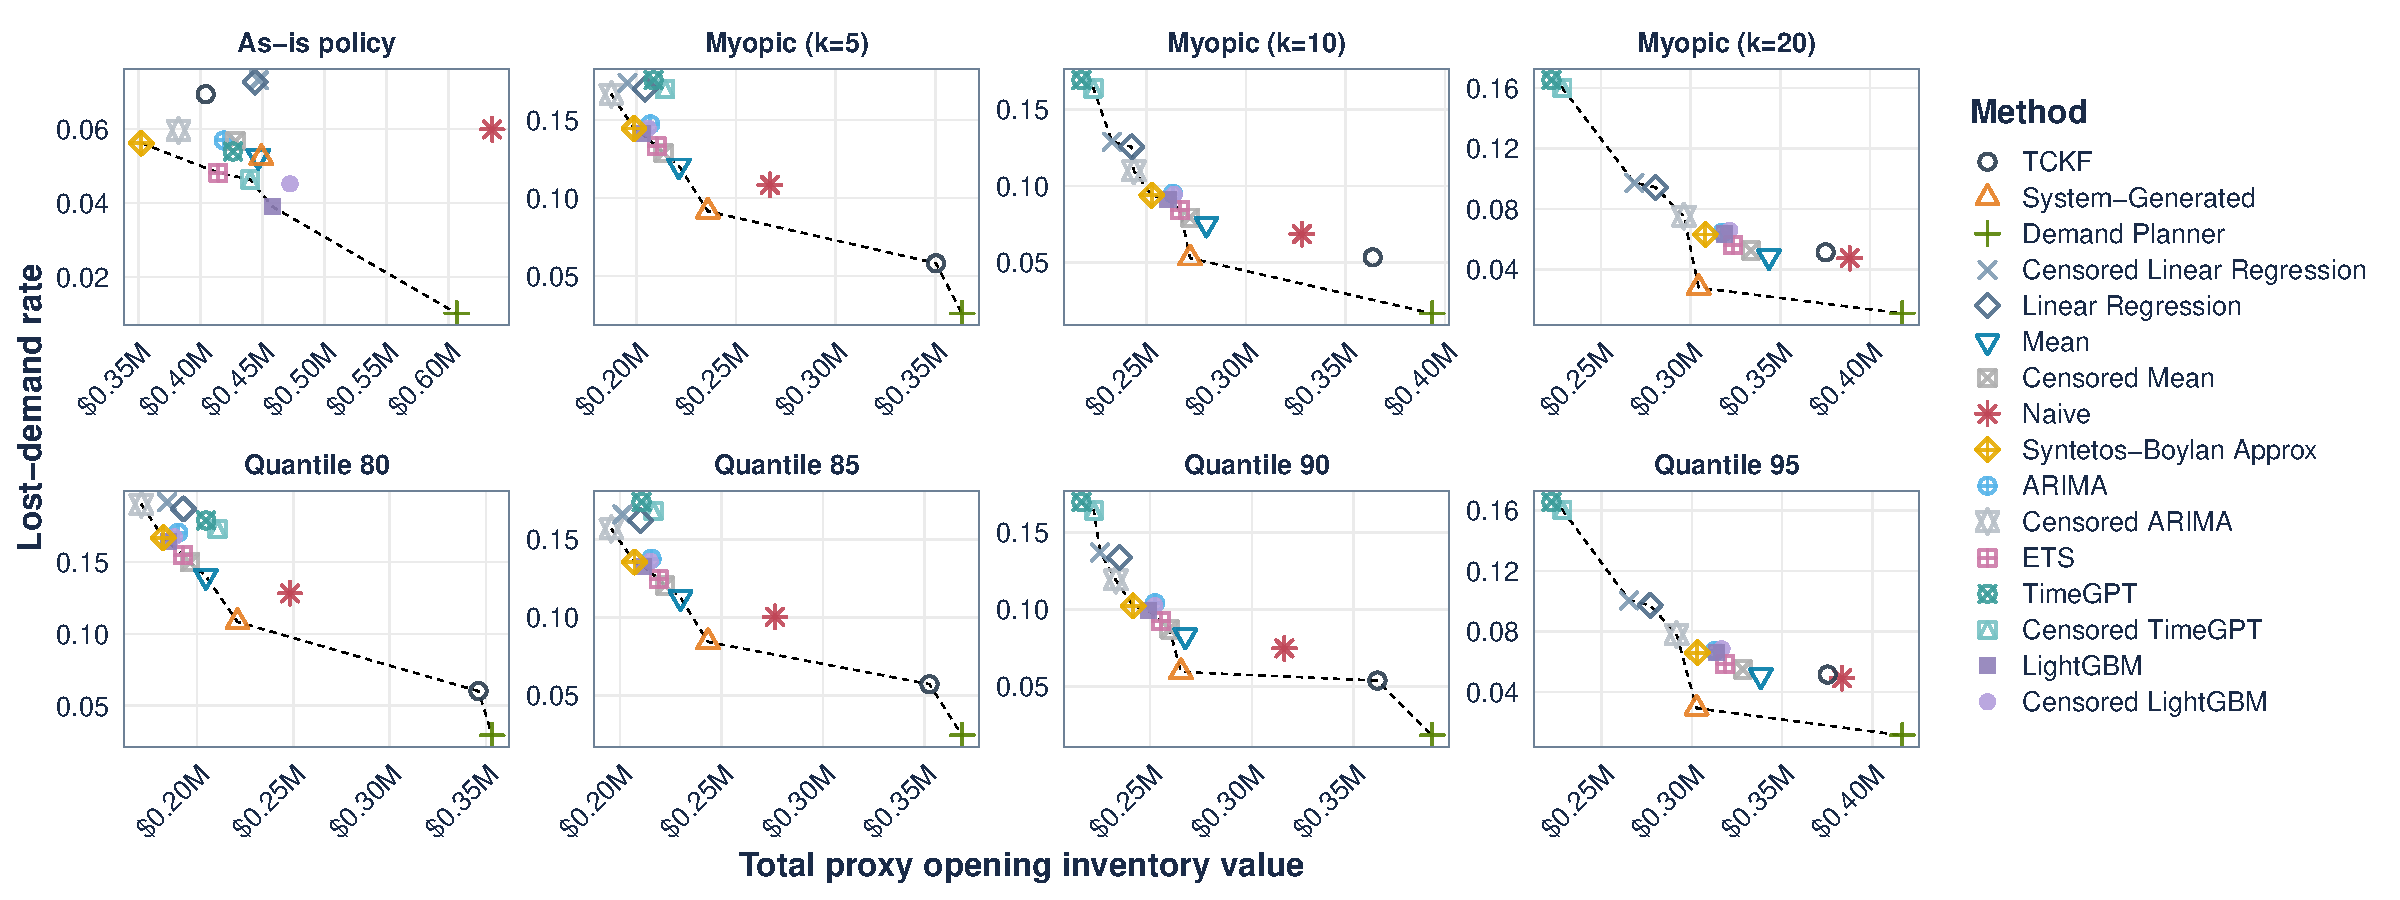
\includegraphics[width=\linewidth,height=0.75\textheight,keepaspectratio]{E-companion-Figure-05.pdf}

}

\caption{\label{fig-emp-lost-demand-proxy-inventory-value}Empirical
inventory trade-off between lost-demand rate and total proxy opening
inventory value across replenishment policies.}

\end{figure}%

\pagebreak

\subsubsection{Examples under the as-is
policy}\label{examples-under-the-as-is-policy}

The as-is policy result also clarifies where TCKF is limited. The as-is
policy applies a fixed multiplier to the point forecast and does not use
the forecast uncertainty generated by TCKF. This is particularly
important for sparse, zero-inflated, and bursty products. For these
products, a three-month multiplier applied to a low mean forecast can
still produce a low absolute stock target, leaving limited protection
against occasional demand spikes. For example, \emph{Copper T IUD} has
very low average demand and a high share of zero-demand months. Under
the as-is policy, TCKF achieves a CSL of 0.647 with an opening stock
position of only 0.26 months of supply, and the lost-demand rate is
0.982. \emph{Implanon} shows a similar but less extreme pattern: TCKF
achieves a CSL of 0.848, with 2.84 opening months of stock and a
lost-demand rate of 0.201. These examples show that the as-is policy can
convert sparse mean forecasts into insufficient stock targets.
Therefore, weaker as-is policy performance should be interpreted as a
limitation of applying a mean-based multiplier to intermittent demand,
rather than as a general failure of TCKF. Although CSL and lost-demand
rate generally show similar service-inventory patterns, we retain
lost-demand rate as a complementary measure because it can reveal
substantial unmet demand during the relatively few positive-demand
periods of sparse and intermittent series.

\subsection{Section 9: Observed product availability from the LMIS stock
movement data}\label{sec-appendix_wp2_6_b}

\begingroup\fontsize{8}{10}\selectfont

\begin{longtable}[t]{>{\raggedright\arraybackslash}p{14em}>{\raggedleft\arraybackslash}p{6em}>{\raggedleft\arraybackslash}p{7em}>{\raggedleft\arraybackslash}p{6em}}

\caption{\label{tbl-emp-inv-true}Observed product availability from the
LMIS stock movement data.}

\tabularnewline

\toprule
Product & Average demand & Average opening stock (MOS) & Achieved CSL\\
\midrule
Overall & 19.73 & 3.98 & 0.838\\
Microgynon / pill (AS27000) & 27.91 & 3.27 & 0.856\\
Microlut (AS27132) & 5.46 & 7.53 & 0.843\\
Depo Provera injectable (AS27133) & 29.43 & 2.83 & 0.790\\
Noristerat injectable (AS27134) & 22.65 & 4.45 & 0.884\\
\addlinespace
Jadelle (AS27137) & 6.28 & 3.23 & 0.917\\
Implanon (AS27138) & 7.82 & 3.04 & 0.748\\
Copper T IUD (AS42018) & 0.75 & 16.73 & 0.896\\
Male condom (AS46000) & 20.46 & 8.91 & 0.923\\
Female condom (AS17005) & 0.42 & 134.49 & 0.956\\
\bottomrule

\end{longtable}

\endgroup{}

\subsection{Section 10: Supporting model
diagnostics}\label{section-10-supporting-model-diagnostics}

\subsubsection{Signal recovery}\label{signal-recovery}

To examine the boundary conditions of TCKF, we first assess its ability
to recover the underlying demand signal under different operational
regimes. Using the numerical dataset, where true demand (\(y_t^*\)) is
known, Figure~\ref{fig-model_diag1_wp2} compares TCKF point predictions
(\(\hat{y}_t\)) with true demand under normal operations, stockouts, and
service interruptions.

\begin{figure}

\centering{

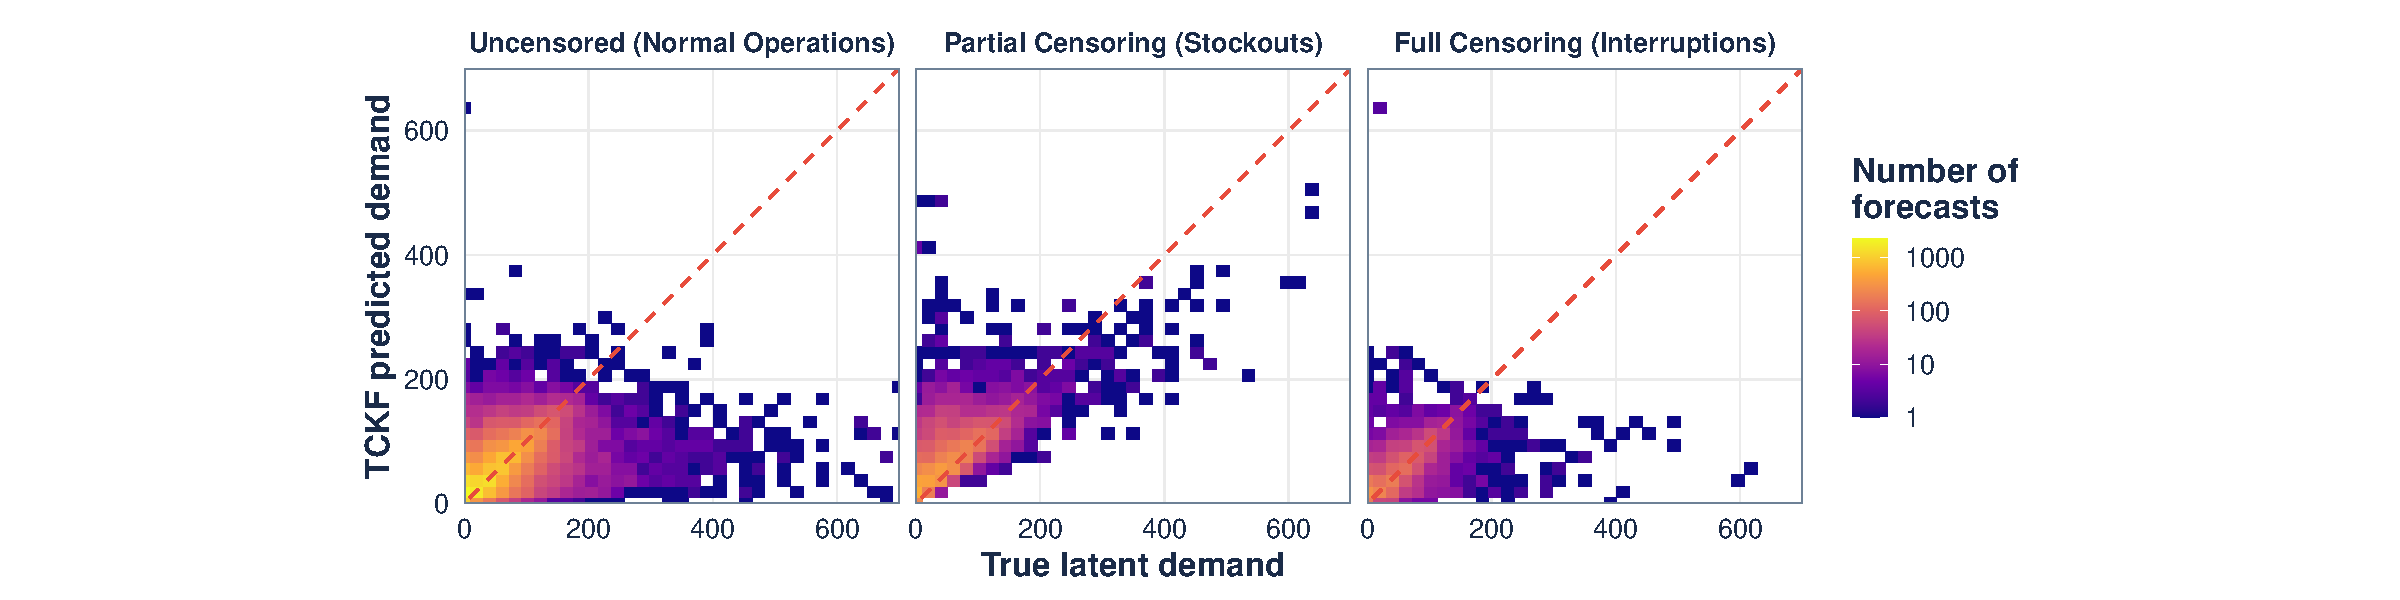
\includegraphics[width=\linewidth,height=0.75\textheight,keepaspectratio]{E-companion-Figure-06.pdf}

}

\caption{\label{fig-model_diag1_wp2}Evaluating signal recovery across
different operational disruptions.}

\end{figure}%

Figure~\ref{fig-model_diag1_wp2} shows a clear but nuanced recovery
pattern. TCKF smooths highly erratic demand and therefore does not fully
recover isolated extreme observations. However, under stockouts, the
truncated Gaussian update uses the available-stock threshold to adjust
the demand estimate upward. During service interruptions, skipping the
measurement update prevents the recorded zero from pulling the state
downward. Thus, distinguishing the two censoring mechanisms helps
preserve the underlying demand signal and avoids the spiral-down effect.

\subsubsection{Model specification, uncertainty inflation and
calibration}\label{model-specification-uncertainty-inflation-and-calibration}

We evaluate how TCKF's internal design choices affect the trade-off
between point accuracy and interval calibration.
Figure~\ref{fig-model_diag2_wp2} summarises the performance of
alternative state specifications, uncertainty-inflation settings, and
conformal calibration schemes.

\begin{figure}

\centering{

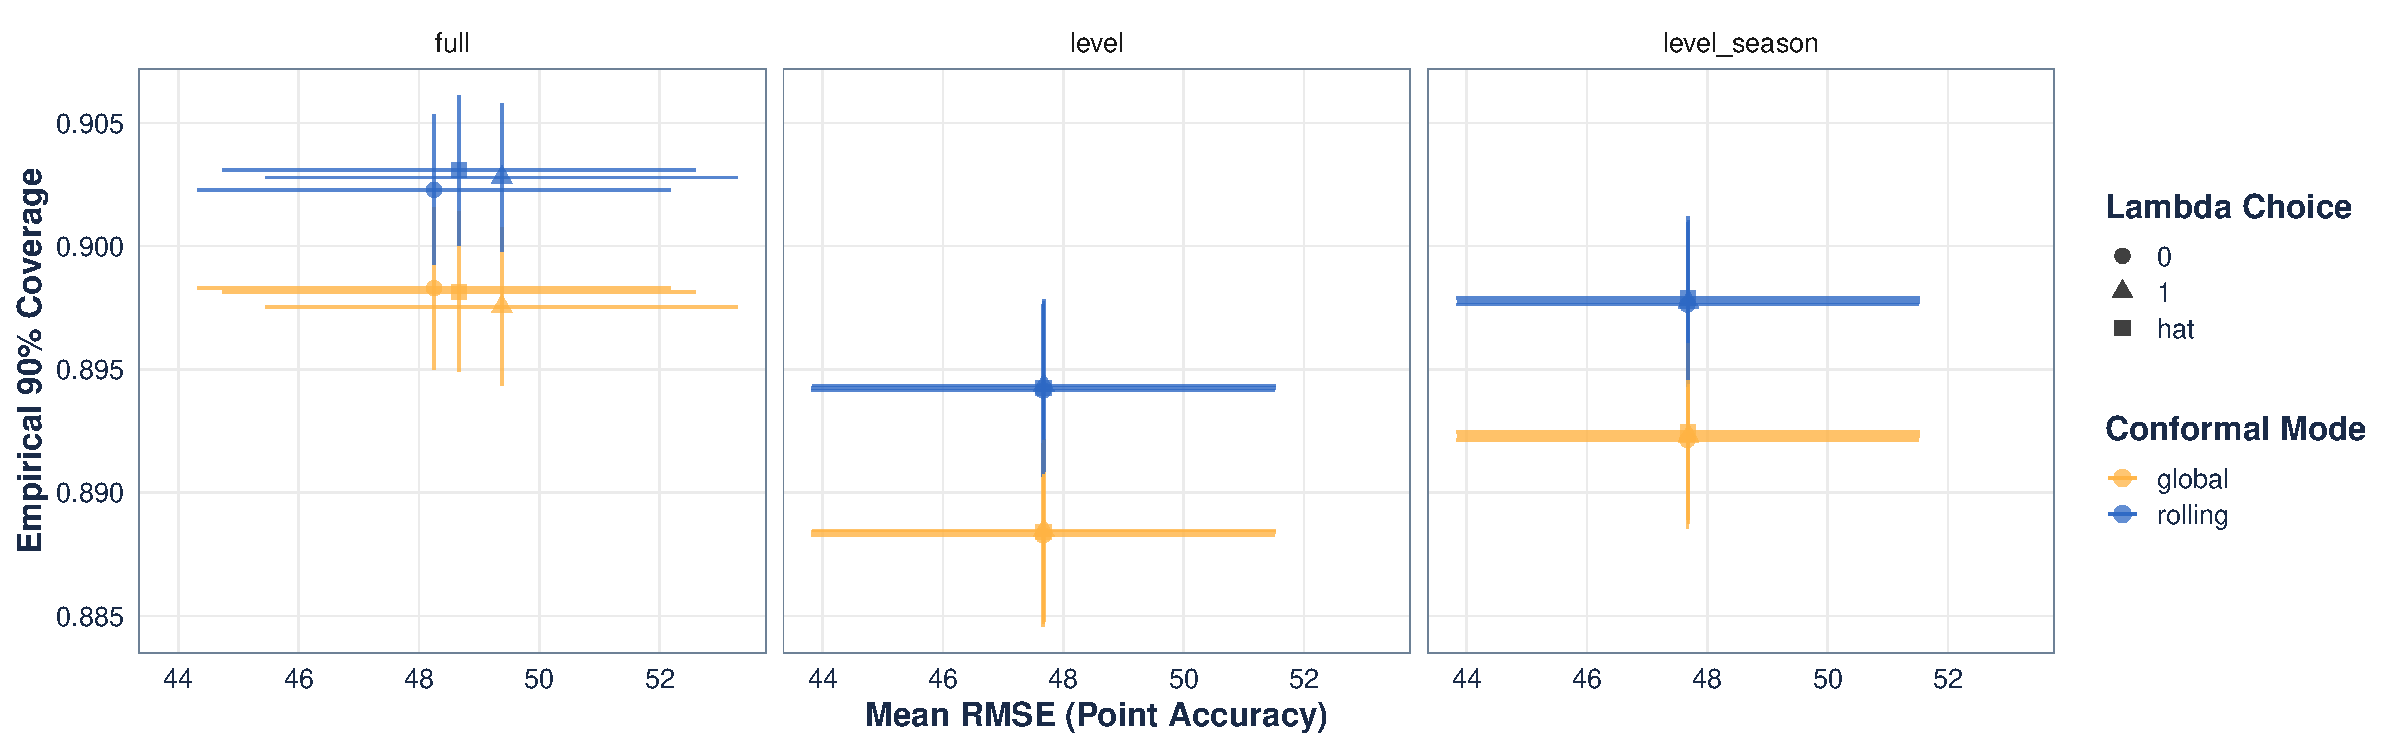
\includegraphics[width=\linewidth,height=0.75\textheight,keepaspectratio]{E-companion-Figure-07.pdf}

}

\caption{\label{fig-model_diag2_wp2}Accuracy-calibration trade-off
induced by the internal modelling choices.}

\end{figure}%

Three findings emerge. First, parsimonious state specifications achieve
equivalent or better RMSE than more complex variants. Second, rolling
conformal calibration improves empirical coverage without materially
affecting point accuracy. Third, dynamically estimating the
uncertainty-inflation weight (\(\hat{\lambda}\)) maintains coverage
while keeping RMSE stable. Together, these results support the
parsimonious and adaptive design choices used in the final TCKF
specification.

\pagebreak

\section*{References}\label{references}
\addcontentsline{toc}{section}{References}

\renewcommand{\bibsection}{}
\bibliography{references.bib}





\end{document}
